\documentclass[9pt,xcolor=x11names,compress]{beamer}

%%% Author and title
\newcommand{\titleinfo}{Using Analysts' Forecasts for Stock Predictions - An Entropic Tilting Approach}
\title{\titleinfo}
\def\authorA{Christoph Frey}
\def\affiliationA{Erasmus University Rotterdam} 
\def\emailA{\href{mailto:christoph.frey@gmail.com}{christoph.frey@gmail.com}}
\newcommand{\authorinfo}{\authorA}

%%% General Packages
\usepackage[english]{babel} 
\usepackage[OT1]{fontenc}
\usepackage[utf8]{inputenc}
\usepackage{color}
\usepackage{graphicx}
\usepackage{caption}

%%%%%%%%%%%%%%
%%% Beamer Layout %%%
%%%%%%%%%%%%%%

%%% Default Theme
\usetheme{default}
\usefonttheme{professionalfonts}

%%% Font Family
\usepackage{cmbright}

%%% No Navigation Bar
\setbeamertemplate{navigation symbols}{}

%%% Transparent uncover with \pause
\setbeamercovered{transparent}

%%% Colors
\definecolor{dblue}{RGB}{40,40,110} %blue
\definecolor{dgreen}{RGB}{10,140,70} %green
\definecolor{dred}{RGB}{180,30,30} %red

\setbeamercolor{frametitle}{fg=dblue}
\setbeamercolor{button}{bg=dblue,fg=white}
\setbeamertemplate{section in head/foot}{\textcolor{dblue}{\hfill\insertsectionhead}}
\setbeamertemplate{section in head/foot shaded}{\textcolor{black!15}{\hfill\insertsectionhead}} % faded section titles for inactive sections

% Colored Links
\usepackage{hyperref}
\hypersetup{colorlinks=true,citecolor=dblue,pdfpagelabels=TRUE,pdfstartview={FitH},linkcolor=dblue,urlcolor=dblue}

%%% Headline
\setbeamerfont{headline}{size=\fontsize{6.5}{1},shape=\scshape}
\setbeamertemplate{headline}{
	\vspace{0.015\paperheight}
	{\leavevmode
		\begin{beamercolorbox}{section in head/foot} 
			\insertsectionnavigationhorizontal{\paperwidth}{\hspace*{0.1ex}}{\hspace*{0.1ex}}
		\end{beamercolorbox}%
		\vspace{0.005\paperheight}}
	\begin{beamercolorbox}[center]{}
		\hspace{0.025\paperwidth}\rule{0.95\paperwidth}{0.5pt}\hspace{0.025\paperwidth}
	\end{beamercolorbox}%
}

%%% Footline
\setbeamerfont{footline}{size=\fontsize{6.5}{1},shape=\scshape}
\setbeamertemplate{footline}{
	\begin{beamercolorbox}[center]{}
		\hspace{0.025\paperwidth}\rule{0.95\paperwidth}{0.5pt}\hspace{0.025\paperwidth}
	\end{beamercolorbox}%
	\leavevmode
	\begin{beamercolorbox}[wd=.5\paperwidth,ht=2.8ex,left]{}
		\hspace*{0.025\paperwidth}\textcolor{dblue}{\insertsubsectionhead}
	\end{beamercolorbox}%
	\begin{beamercolorbox}[wd=.5\paperwidth,ht=2.8ex,right]{}
		\insertframenumber{} $|$ \inserttotalframenumber \hspace{0.025\paperwidth} 
	\end{beamercolorbox}%
	\vspace{0.015\paperheight}
}

%%% Itemize / Enumerate Symbols
\setbeamertemplate{itemize items}{\textcolor{dblue}{\raisebox{0.6pt}{\footnotesize$\blacktriangleright$}}}
\setbeamertemplate{itemize subitem}{\textcolor{dblue}{\raisebox{0.6pt}{\footnotesize$\triangleright$}}}
\setbeamertemplate{itemize subsubitem}{\textcolor{dblue}{\raisebox{0.6pt}{\footnotesize$\bullet$}}}
\setbeamertemplate{enumerate items}{\textcolor{dblue}{\raisebox{0.6pt}{\footnotesize\insertenumlabel.}}}

%%% Title Page
\setbeamertemplate{title page}{%
	\vspace*{0.1\paperheight}
	\fontsize{14}{20}\selectfont{\color{dblue}{\inserttitle}}
	\vskip1em\par
	\fontsize{10}{11}\selectfont{\authorA}
	\vskip0.5em\par
	\fontsize{9}{11}\selectfont{\hspace{0cm} \affiliationA\vskip1mm\par
	\hspace{0cm} \emailA}\vskip1mm\par
	\vskip5em\par
	\begin{figure}
		\today\hfill\includegraphics[height=0.125\linewidth]{signature.pdf}\hspace{.5cm}
	\end{figure}
}
%%% New Commands

% Text Color Commands
\newcommand{\btext}{\textcolor{dblue}}
\newcommand{\bbtext}[1]{\textcolor{dblue}{\textbf{#1}}}
\newcommand{\rtext}{\textcolor{dred}}
\newcommand{\rbtext}[1]{\textcolor{dred}{\textbf{#1}}}
\newcommand{\gtext}{\textcolor{dgreen}}
\newcommand{\gbtext}[1]{\textcolor{dgreen}{\textbf{#1}}}

% Enumerate Counter
%\newcounter{saveenumi}
%\newcommand{\seti}{\setcounter{saveenumi}{\value{enumi}}} % save current counter
%\newcommand{\conti}{\setcounter{enumi}{\value{saveenumi}}} % continue current counter

% Set Introduction = section 0
\setcounter{section}{-1}

% Bibliography
\usepackage{hyperref}
\usepackage{nameref}
\usepackage[labelformat=empty]{caption}
\usepackage[sectionbib]{natbib}
\let\natbibcitet\citet
\renewcommand\citet{\bibpunct{(}{)}{,}{a}{,}{,}\natbibcitet}
\let\natbibcitep\citep
\renewcommand\citep{\bibpunct{(}{)}{;}{a}{,}{;}\natbibcitep}

\let\oldcite=\cite                                                              
\renewcommand{\cite}[1]{\textcolor{dblue}{\oldcite{#1}}}

%%% Blocks
\usepackage{tcolorbox}
\tcbuselibrary{theorems}

% Definition (blue)
%\newtcolorbox[auto counter, number within=section]{defbox}[2][]{colback=dblue!2,colframe=dblue!30!black,coltitle=dblue,colbacktitle=dblue!10!white,before=\begin{center},after=\end{center},width=0.9\textwidth,left=3pt,right=3pt,toptitle=3pt,bottomtitle=3pt,boxrule=0.2mm,fonttitle=\bfseries,title={Definition~\thetcbcounter: #2},#1}
\newtcolorbox[auto counter, number within=section]{defbox}[2][]{colback=dblue!2,colframe=dblue!30!black,coltitle=dblue,colbacktitle=dblue!10!white,before=\begin{center},after=\end{center},width=0.9\textwidth,left=3pt,right=3pt,toptitle=3pt,bottomtitle=3pt,boxrule=0.2mm,fonttitle=\bfseries,title={Definition},#1}
% Proposition (green)
\newtcolorbox[auto counter, number within=section]{propbox}[2][]{colback=dgreen!2,colframe=dgreen!30!black,coltitle=dgreen,colbacktitle=dgreen!10!white,before=\begin{center},after=\end{center},width=0.9\textwidth,left=3pt,right=3pt,toptitle=3pt,bottomtitle=3pt,boxrule=0.2mm,fonttitle=\bfseries,title={Proposition},#1}
% Blue box
\newtcolorbox{bbox}[2][]{colback=dblue!2,colframe=dblue!30!black,coltitle=dblue,colbacktitle=dblue!10!white,before=\begin{center},after=\end{center},width=0.9\textwidth,left=3pt,right=3pt,toptitle=3pt,bottomtitle=3pt,boxrule=0.2mm,fonttitle=\bfseries,title={#2},#1}
% Red Box
\newtcolorbox{rbox}[2][]{colback=dred!2,colframe=dred!30!black,coltitle=dred,colbacktitle=dred!10!white,before=\begin{center},after=\end{center},width=0.9\textwidth,left=3pt,right=3pt,toptitle=3pt,bottomtitle=3pt,boxrule=0.2mm,fonttitle=\bfseries,title={#2},#1}
% Green Box
\newtcolorbox{gbox}[2][]{colback=dgreen!2,colframe=dgreen!30!black,coltitle=dgreen,colbacktitle=dgreen!10!white,before=\begin{center},after=\end{center},width=0.9\textwidth,left=3pt,right=3pt,toptitle=3pt,bottomtitle=3pt,boxrule=0.2mm,fonttitle=\bfseries,title={#2},#1}

\definecolor{pbblue}{HTML}{0A75A8}% color for the progress bar and the circle

\usepackage{booktabs}

%%%%%%%%%%%%%%%%%%%%%%%
%%% Special Content %%%
%%%%%%%%%%%%%%%%%%%%%%%
\newtheoremstyle{standard}% name
{0,5cm}      % Space above
{0,5cm}      % Space below
{\upshape} % Body font
{}         % Indent amount (empty = no indent, \parindent = para indent)
{\bfseries}% Thm head font
{}        % Punctuation after thm head
{\newline} % Space after thm head: " " = normal interword space;
% \newline = linebreak
{}         % Thm head spec (can be left empty, meaning `normal')
%
\theoremstyle{standard}
\newtheorem{lem}{Lemma}[section]
\newtheorem{defi}{Definition}[section]
\newtheorem{theo}{Theorem}[section]
\newtheorem{prop}{Proposition}[section]
\newtheorem{assu}{Assumption}[section]
\newtheorem{excu}{Excursus}[section]
\newtheorem{prf}{Proof}[section]
%
%
\newtheoremstyle{notes}% name
{0.5cm}      % Space above
{0.5cm}      % Space below
{} % Body font
{}         % Indent amount (empty = no indent, \parindent = para indent)
{\itshape}% Thm head font
{}        % Punctuation after thm head
{\newline} % Space after thm head: " " = normal interword space;
% \newline = linebreak
{}         % Thm head spec (can be left empty, meaning `normal')
%
\theoremstyle{notes}
\newtheorem{exam}{Example}[section]
\newtheorem{nota}{Notation}[section]
\newtheorem{rema}{Remark}[section]
\newtheorem{hypo}{Hypothesis}
\newtheorem{exerc}{\large{Exercise}}[subsection]
\newtheorem{exerc1}{\large{Exercise}}[section]

% Enumerate Counter
\newcounter{saveenumi}
\newcommand{\seti}{\setcounter{saveenumi}{\value{enumi}}}
\newcommand{\conti}{\setcounter{enumi}{\value{saveenumi}}}
% New Envirmoments
%\newcommand{\argmin}{\arg\!\min}
%\newcommand{\argmax}{\arg\!\max}

\newcommand{\am}[1]{\underset{#1}{\rm arg \, min } \,}
% arg min über {}
\newcommand{\amx}[1]{\underset{#1}{\rm arg max } \,}
% arg max über {}

% argmin, argmax
\newcommand{\argmin}[1]{\underset{#1}{\rm arg \, min } \,}
\newcommand{\argmax}[1]{\underset{#1}{\rm arg max } \,}


% Frieder's commands
%\newcommand{\N}[2]{\text{N} \left( \, #1 \, , \, #2 \, \right)}
\newcommand{\No}[1]{\text{N}\hspace{-0.05cm}\left(#1\right)}
\newcommand{\Ex}[1]{\text{E}\hspace{-0.05cm}\left(#1\right)}
\newcommand{\cov}[1]{\text{cov}\hspace{-0.05cm}\left(#1\right)}

%\newcommand{\IG}[2]{\text{IG} \left( \, #1 \, , \, #2 \, \right)}
\newcommand{\IG}[2]{\text{IG} \left( \, #1 \, , \, #2 \, \right)}


% Ingmar's commands
\DeclareMathOperator*{\pr}{Pr}
\newcommand{\p}[1]{\pr \left[ #1 \right]}
\newcommand{\pc}[2]{\pr \left[ #1 \left| #2 \right.\right]}
\newcommand{\pci}[3]{\pr_#3 \left[ #1 \left| #2 \right.\right]}
\DeclareMathOperator*{\Ew}{E}
\DeclareMathOperator*{\ewd}{\hat E}
\newcommand{\ew}{{\Ew}}
\newcommand{\e}[1]{\ensuremath{\Ew \left[ {#1} \right]}}
\newcommand{\edach}[1]{\ensuremath{\ewd \left[{#1} \right]}}
\newcommand{\ec}[2]{\Ew \left[ \left. #1 \right| #2 \right]}
\DeclareMathOperator*{\var}{V}
\newcommand{\va}[1]{\var\left[ {#1} \right]}
\newcommand{\vc}[2]{\var \left[ \left. #1 \right| #2 \right]}
\newcommand{\estvar}[1]{ \hat{\var} \left[ #1 \right]}
\DeclareMathOperator*{\cova}{Cov} \DeclareMathOperator*{\cor}{Corr}
%\newcommand{\cov}[1]{{\cova}\left[ {#1} \right]}
\newcommand{\corr}[1]{{\cor}\left[ {#1} \right]}
\newcommand{\no}[1]{{\rm N} \left( #1 \right)}
\newcommand{\nor}{\rm N}
\newcommand{\iidno}[1]{{\rm \stackrel{iid}{\sim} N} \left( #1 \right)}
\newcommand{\nv}[1]{\Phi \left( #1 \right)}
\DeclareMathOperator*{\median}{median} \DeclareMathOperator*{\mini}{min}
\DeclareMathOperator*{\maxi}{max}
\newcommand{\set}{\mathbb}
\newcommand{\setdef}[3]{\set #1 &:=& \left\{ #2 \quad : \quad #3 \right\}}
\newcommand{\plimn}{\underset{N\rightarrow \infty}{\rm plim } \quad }
\newcommand{\plimt}{\underset{T\rightarrow \infty}{\rm plim } \quad }
\newcommand{\plim}{\mathrm{p}\hspace*{-3pt}\lim\limits}
\newcommand{\pd}[2]{ \frac{\partial #1}{\partial #2}}


\newcommand{\Tab}[4]{
	\begin{center}
		$
		\begin{array}{c}
		\text{#1} \\
		\text{ \parbox[t]{#4}{\vspace*{0,05cm}\footnotesize{\refstepcounter{table}{\bf Table \thetable: \hspace*{-0.25cm} #3}
					#2}}}
		\end{array}
		$
	\end{center}
}

\newcommand{\TabC}[4]{\addtocounter{table}{-1}
	\begin{center}
		$
		\begin{array}{c}
		\text{#1} \\
		\text{ \parbox[t]{#4}{\vspace*{0,05cm}\footnotesize{\refstepcounter{table}{\bf Table \thetable~(cont'd): \hspace*{-0.25cm} #3}
					#2}}}
		\end{array}
		$
	\end{center}
}

\newcommand{\TabT}[5]{
	\begin{center}
		$
		\begin{array}{l}
		\text{#1} \\
		\text{#2} \\
		\text{ \parbox[t]{#5}{\vspace*{0,05cm}\footnotesize{\refstepcounter{table}{\bf Table \thetable: \hspace*{-0.25cm}#4}
					#3}}}
		\end{array}
		$
	\end{center}
}

\newcommand{\Fig}[4]{
	\begin{center}
		$
		\begin{array}{l}
		#1 \\
		\text{ \parbox[t]{#4}{\vspace*{0,1cm}\footnotesize{\refstepcounter{figure}{\vspace*{-0.5cm} {\bf Figure \thefigure:} \hspace*{-0.15cm} #3} #2}}}
		\end{array}
		$
	\end{center}
}

\newcommand{\FigC}[4]{\addtocounter{figure}{-1}
	\begin{center}
		$
		\begin{array}{l}
		#1 \\
		\text{ \parbox[t]{#4}{\vspace*{0,1cm}\footnotesize{\refstepcounter{figure}{\vspace*{-0.5cm} {\bf Figure \thefigure~(cont'd).} \hspace*{-0.15cm} #3} #2}}}
		\end{array}
		$
	\end{center}
}



% % % New Commands?

\newcommand{\beq}{\begin{equation}}
\newcommand{\eeq}{\end{equation}}
\newcommand{\beqno}{\begin{equation*}}
\newcommand{\eeqno}{\end{equation*}}
\newcommand{\beqn}{\begin{eqnarray}}
\newcommand{\eeqn}{\end{eqnarray}}
\newcommand{\beqnn}{\begin{eqnarray*}}
	\newcommand{\eeqnn}{\end{eqnarray*}}
\newcommand{\balgn}{\begin{align}}
\newcommand{\ealgn}{\end{align}}
\newcommand{\balgnn}{\begin{align*}}
\newcommand{\ealgnn}{\end{align*}}
%\newcommand{\si}{\sigma}
\newcommand{\nono}{\nonumber}
\newcommand{\mbb}{\mathbb}
\newcommand{\mca}{\mathcal}
\newcommand{\msc}{\mathscr}
\newcommand{\ben}{\begin{enumerate}}
	\newcommand{\een}{\end{enumerate}}
\newcommand{\bit}{\begin{itemize}}
	\newcommand{\eit}{\end{itemize}}
\newcommand{\lhs}{\hspace{0.4cm}}
\newcommand{\shs}{\hspace{0.2cm}}
\newcommand{\lvs}{\vspace{0.4cm}}
\newcommand{\svs}{\vspace{0.2cm}}
\newcommand{\mbbe}{\mathbb{E}}
\newcommand{\mbbv}{\mathbb{V}}
\newcommand{\mbbcv}{\mathbb{CV}}
\newcommand{\mc}{\multicolumn}
\newcommand{\bbm}{\begin{bmatrix}}
	\newcommand{\ebm}{\end{bmatrix}}
\newcommand{\lf}{\lfloor}
\newcommand{\rf}{\rfloor}

\newcommand{\VEC}{\text{vec}}
%\newcommand{\E}{\text{E}}
\newcommand{\V}{\text{V}}

\newcommand{\hilit}[1]{ \textcolor{green}{\textbf{#1}}}

\begin{document}
%\fontsize{8}{12}\selectfont{
\section{Introduction}
\begin{frame}[plain,noframenumbering]
\titlepage
\end{frame}
%%%%%%%%%%%%%%%%%%%%%%%%%%%
%%%%%%%%%%%%%%%%%%%%%%%%%%%

\begin{frame}{Motivation}
	\begin{itemize}
		\item Predicting asset returns is a popular exercise in finance
		\item Challenging task because of (i) estimation and model uncertainty, (ii) a substantial unpredictable component (shocks) in future stock returns and (iii) model exploitation by other market participants
		\item Recent evidence for predictability: model averaging \cite{pettenuzzo2016}, time-varying-parameters \cite{dangl2012}, stochastic volatility and predictive distributions \cite{johannes2014}
	\end{itemize}
\pause
\textbf{But}
\begin{itemize}
	\item Most prediction models relate the future stock returns to past observations of asset specific variables such as the dividend yield
	\item Stock price is forward-looking as it reflects the expectations of market participants about the future cash flows
	\item In this paper, use forward-looking information (professional analyst forecasts) to make stock return predictions
	\item Approach similar to \cite{metaxoglou2016}, who improve equity premium forecasts by using option prices
\end{itemize}
\end{frame}
%%%%%%%%%%%%%%%%%%%%%%%%%%%
%%%%%%%%%%%%%%%%%%%%%%%%%%%

\begin{frame}{Motivation - IBM Stock Price}
\begin{figure}
	\centering
	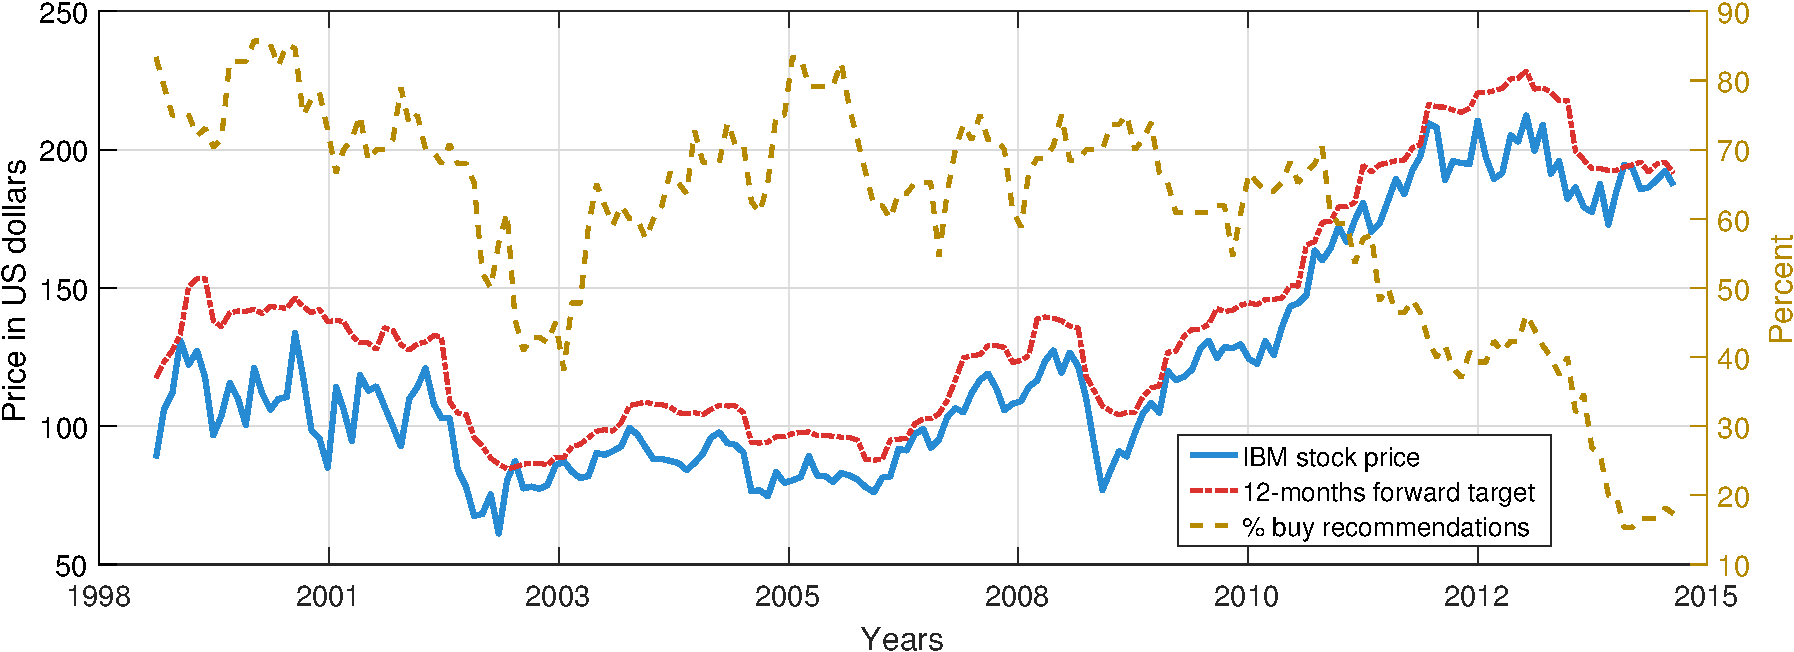
\includegraphics[width=1\linewidth]{../../Tex/plots/IBM_price_plot}
	\label{fig:ibmpriceplot}
\end{figure}

\end{frame}
%%%%%%%%%%%%%%%%%%%%%%%%%%%
%%%%%%%%%%%%%%%%%%%%%%%%%%%

\begin{frame}{Motivation - IBM Return Prediction}
	\begin{figure}
		\centering
		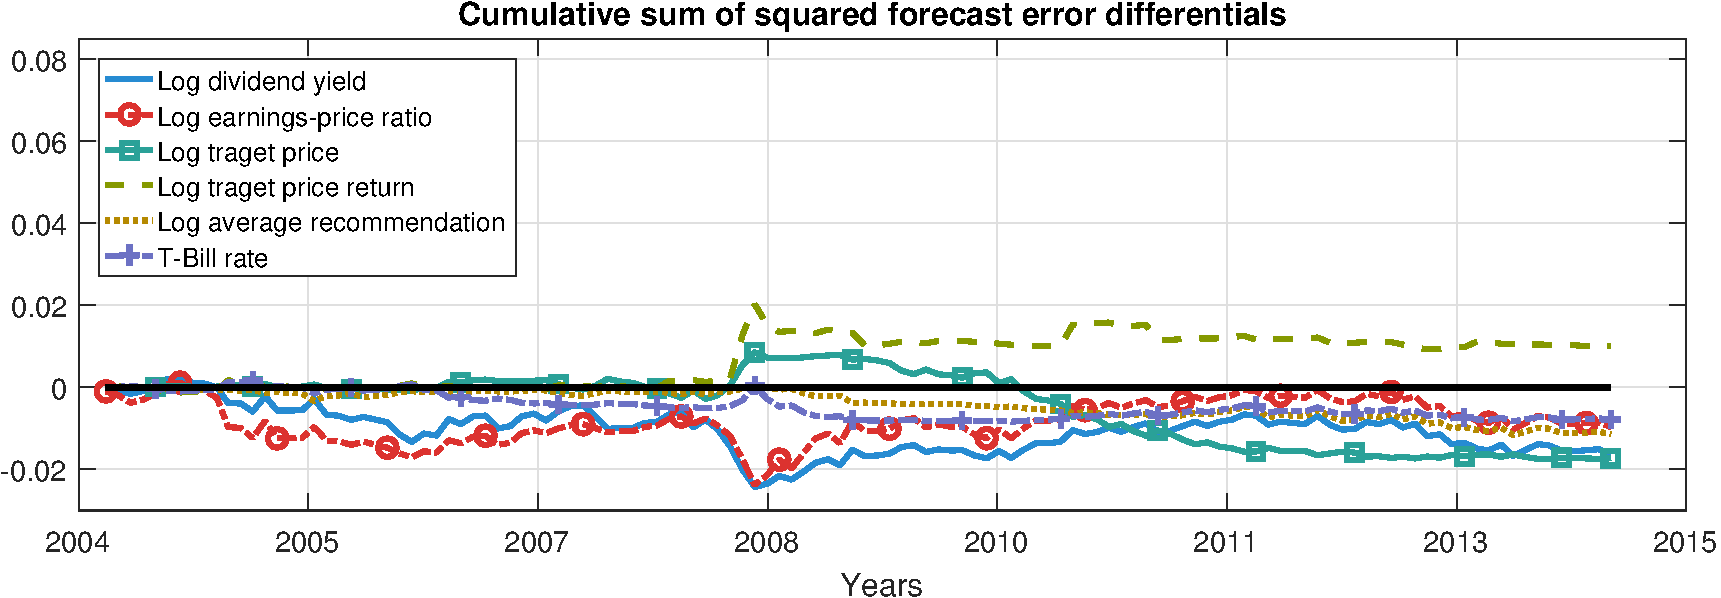
\includegraphics[width=1\linewidth]{../../Tex/plots/IBM_CSSED_plot}\\
		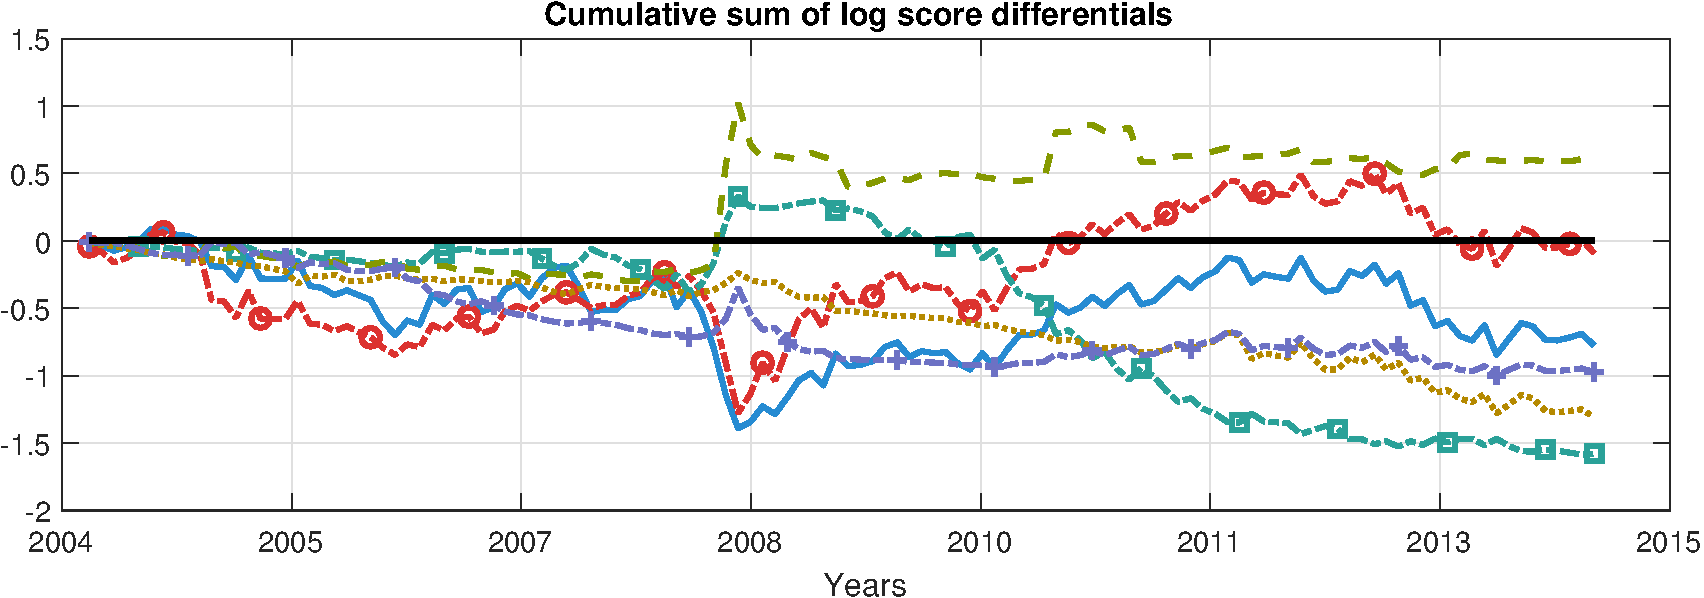
\includegraphics[width=1\linewidth]{../../Tex/plots/IBM_CLSD_plot}\\
		\label{fig:ibmpredplot}
	\end{figure}
\end{frame}
%%%%%%%%%%%%%%%%%%%%%%%%%%%
%%%%%%%%%%%%%%%%%%%%%%%%%%%

\begin{frame}{Contributions}
	In this paper, 
	\begin{itemize}
		\item we adopt the so-called \bbtext{forgetting factors} approach of \cite{koop2013} which allows for all the features recently found to be important to find significant return predictability: Time-varying parameters, stochastic volatility, parameter shrinkage as well as dynamic model averaging and variable selection
		\pause
		\item we use the (dis-)agreement in the analysts' forecast to regularize/reweight the predictive return distribution via by a method called \bbtext{entropic (exponential) tilting}
		\pause
		\item we restrict the mean and variance of the predictive distribution to coincide with the mean and the variance of monthly target price implied expected returns, i.e. simple returns between the current spot and the target price
		\pause
		\item we find that restricting the variance of the asset returns is beneficial in terms of out-of-sample performance, as it provides a forward looking measure for (un-)certainty in the market
	\end{itemize}
\end{frame}
%%%%%%%%%%%%%%%%%%%%%%%%%%%
%%%%%%%%%%%%%%%%%%%%%%%%%%%

\begin{frame}{Motivation - Analysts Recommendations}
\textbf{How informative are sell-side based analyst forecasts for return prediction?}
\begin{itemize}
	\item \cite{ramnath2008}: HUGE literature about shortcomings of analyst forecasts: Incentives and biases, information content and market inefficiencies, mostly related to accounting figures (earnings forecasts)
\end{itemize}
\pause\bbtext{Analysts recommendations}
\begin{itemize}
	\item \cite{barber2001,green2006, cvitanic2006} report abnormal returns from trading strategies that go long in stocks with favorable recommendations and short in stocks with unfavorable ratings
	%\item \cite{cvitanic2006} shows that simple long-short portfolios can be outperformed by multi-period expected utility maximizing strategies using analysts recommendations
	%\item \cite{he2013}: Stocks with favorable (unfavorable) recommendations on average outperformed (underperformed) the benchmark index
\end{itemize}
\pause\bbtext{Twelve months forward target price}
\begin{itemize}
	\item \cite{brav2003} show that there are substantial short-term market reactions in the stock price to target changes
	%\item \cite{bradshaw2012b} find an average target price premium over the spot price of 15 percent
	\item \cite{da2011} find that aggregating stocks across sectors according to their twelve month forward target price implied expected return, i.e. simple return between the current and the target price, yields significant risk-adjusted abnormal returns for different long-short portfolio
\end{itemize}
\end{frame}
%%%%%%%%%%%%%%%%%%%%%%%%%%%
%%%%%%%%%%%%%%%%%%%%%%%%%%%

%\begin{frame}{Motivation - Target Prices}
%\bbtext{Twelve months forward target price}
%	\begin{itemize}
%		\item \cite{brav2003} show that there are substantial short-term market reactions in the stock price to target changes
%		\item \cite{bradshaw2012b} find an average target price premium over the spot price of 15 percent
%		\item \cite{da2011} find that aggregating stocks across sectors according to their twelve month forward target price implied expected return, i.e. simple return between the current and the target price, yields significant risk-adjusted abnormal returns for different long-short portfolio
%	\end{itemize}
%\end{frame}
%%%%%%%%%%%%%%%%%%%%%%%%%%%%
%%%%%%%%%%%%%%%%%%%%%%%%%%%%

\begin{frame}{Outline of the Talk}
	\begin{itemize}
		\item Prediction model
		\item Entropic tilting \citep{krueger2015}
		\item Financial Analysts' data
		\item Empirical application with 20 Dow Jones constituents
		\item Conclusions
	\end{itemize}
\end{frame}
%%%%%%%%%%%%%%%%%%%%%%%%%%%
%%%%%%%%%%%%%%%%%%%%%%%%%%%

\section{Prediction model}

\begin{frame}{Prediction Model I}
	\begin{itemize}
		\item \cite{kandel1987} propose a vector autoregression formulation to jointly model the dynamics of asset returns and its predictor:
		\begin{align}
		\label{eqn:ks1987}
		r_{t+1}&=a_r+b_rx_t+\varepsilon_{r,t+1},\\
		x_{t+1}&=a_x+b_xx_t+\varepsilon_{x,t+1},\label{eqn:ks1987_2}
		\end{align}
		\item the excess return and the predictor variable, only depend on their own lag
		\item Formulation for $K$ predictor variables:
		\begin{align}\label{eqn:varp}
		\begin{bmatrix}r_t\\x_t\end{bmatrix}=a+\sum_{i=1}^pA_i\begin{bmatrix}r_{t-i}\\x_{t-i}\end{bmatrix}+\varepsilon_t,\quad t=1,\ldots,T,	
		\end{align}
		where $r_t$ is the excess return of a particular stock, $x_t=[x_{1,t},\ldots,x_{K,t}]'$ is a $K\times1$ vector of predictor variables and $\varepsilon_t\stackrel{iid}{\sim}\No{0,\Sigma}$
	\end{itemize}
\end{frame}
%%%%%%%%%%%%%%%%%%%%%%%%%%%
%%%%%%%%%%%%%%%%%%%%%%%%%%%


\begin{frame}{Prediction model II}
	\begin{itemize}
		\item Restrict the system such that $r_t$ depends on the entire $x_{t-1}$ vector but $x_{k,t}$, $1\leq k\leq K$, only depends on its own lag $x_{k,t-1}$. Compactly, the resulting model is of the form
		\begin{equation}\label{eqn:var1}
		y_t=(r_t,x_t)'=a+A_1y_{t-1}+\varepsilon_t,
		\end{equation}
		where $a=(a_r,a_{x_1},\ldots,a_{x_K})'$ and $$A_1=\begin{pmatrix} 0 & A_1^{1,2}& A_1^{1,3}&\cdots  & A_1^{1,K+1}\\0 & A_1^{2,2} &0& \cdots & 0\\ \vdots&\ddots&A_1^{3,3}&\ddots& \vdots\\\vdots&&\ddots&\ddots&0\\0&\cdots&\cdots&0&A_1^{K+1,K+1}\end{pmatrix}$$
		\item To implement these restrictions on the coefficient matrix $A_1$ we use a variant of the Minnesota prior \citep{doan1984}
	\end{itemize}
\end{frame}
%%%%%%%%%%%%%%%%%%%%%%%%%%%
%%%%%%%%%%%%%%%%%%%%%%%%%%%

\begin{frame}{Prior Model specification for VAR(1) system}
	\begin{itemize}
		\item Independent marginal normal priors for each set of parameters:
		\begin{align}\label{eqn:priora}
		p(a)&\sim\No{0,\zeta\times\text{I}_{(K+1\times K+1)}},\\\label{eqn:priorA11}
		p(A_1^{1,1}) &\sim \No{0,\varrho\times1},\\\label{eqn:priorA1k}
		p(A_1^{1,k}) &\sim \No{0,\zeta\times \frac{\sigma_r^2}{\sigma_{x_k}^2}},\quad k=1,\ldots,K\\\label{eqn:priorAk1}
		p(A_1^{k,1}) &\sim \No{0,\varrho\times \frac{\sigma_{x_k}^2}{\sigma_{r}^2}},\quad k=2,\ldots,K,\\\label{eqn:priorAkl}
		p(A_1^{k,l}) &\sim \No{\underline{A}_1^{k,l},\varrho\times \frac{\sigma_{x_k}^2}{\sigma_{x_l}^2}},\quad k=2,\ldots,K,\quad l=2,\ldots,K\\
		&  \quad\,\,\text{with } \underline{A}_1^{k,l} = d_k \text{ if $k=l$, and $\underline{A}_1^{k,l} = 0$ otherwise.} \nonumber
		\end{align}
		\item $d_k=0$ for real, $d_k=0.8$ for nominal variables, $\varrho=10^{-4}$, $\zeta=0.2$
		\item Prior is centered around zero implying no predictability. 
		\item $\sigma_{x_k}^2$ $\forall k,r$ are approximated by the residual variances of AR(1) regressions
		\item Diffuse prior for $\Sigma, \ p(\Sigma) \propto | \Sigma|^{-2(2M+1)/2}$.
	\end{itemize}
\end{frame}
%%%%%%%%%%%%%%%%%%%%%%%%%%%
%%%%%%%%%%%%%%%%%%%%%%%%%%%

\begin{frame}{Time-varying Bayesian VAR and stochastic volatility}
	\begin{itemize}
		\item Numerous examples favoring equity prediction models with time-varying parameters (TVP) \citep{dangl2012}, stochastic volatility (SV) \citep{johannes2014} and BMA \citep{pettenuzzo2016}
		\item MCMC/simulations methods computational too costly to estimate VAR system with many predictor variables for recursive forecasting
		\item Solution: \textit{forgetting factors} approach of \cite{koop2013} 
		\item Consider a time-varying VAR version of (\ref{eqn:var1}) with stochastic volatility:
		\begin{align}\label{eqn:tvpvar1}
		y_t&=a_t+A_{1,t}\,y_{t-1}+\varepsilon_t,\\
		A_t&=\phi A_{t-1}+(1-\phi)\underline{A}_0+u_t,\label{eqn:tvpvar2}
		\end{align}
		where $A_t=[a_t\,\,\, A_{1,t}]$, $\varepsilon_t\stackrel{iid}{\sim}\No{0,\Sigma_t}$, $u_t\stackrel{iid}{\sim}\No{0,\Omega_t}$ and $\varepsilon_t\perp u_s\forall\,t,s$
		\item $\phi=1$ implies a random walk behavior, $\phi=0$ implies a random behavior of each $A_t$ around $\underline{A}_0$
	\end{itemize}
\end{frame}
%%%%%%%%%%%%%%%%%%%%%%%%%%%
%%%%%%%%%%%%%%%%%%%%%%%%%%%

\begin{frame}{Forgetting factors I}
	\begin{itemize}
		\item Typically, the estimation of (\ref{eqn:tvpvar1}) - (\ref{eqn:tvpvar2}) involves drawing $A_t$ conditional on $\Sigma_t$ and $\Omega_t$ (e.g. through a Kalman filter), then drawing $\Sigma_t$ conditional on $A_t$ and $\Omega_t$, the sampling $\Omega_t$ given $A_t$ and $\Sigma_t$ and eventually drawing further parameters given conditional on $A_t$, $\Sigma_t$, and $\Omega_t$ for all $t$. 
		\item Computationally demanding as it involves simulating $\Sigma_t$, and $\Omega_t$ for every $t=1,\ldots,T$.
		\pause
		\item \rbtext{Idea of the forgetting factors:} avoid simulating $\Omega_t$ in the Kalman filter by approximating the one-step ahead predictor variance of $A_t|y^{t-1}\sim\No{A_{t|t-1},P_{t|t-1}}$, i.e. $P_{t|t-1}$, by the variance of the filtered estimator $A_{t-1}|y^{t-1}\sim\No{A_{t-1|t-1},P_{t-1|t-1}}$, i.e. $P_{t-1|t-1}$, divided by a \textit{forgetting factor} $\lambda\in[0,1]$:
		\begin{align}
		P_{t|t-1}=P_{t-1|t-1}\big/\lambda
		\end{align}
		\item Then approximate $\Omega_t$ by $(\lambda^{-1}-1)P_{t-1|t-1}$.
		\item Further, $\hat{\Sigma}_t=\kappa\hat{\Sigma}_{t-1}+(1-\kappa)\hat{\varepsilon}_t\hat{\varepsilon}_t'$, where $\hat{\varepsilon}_t=y_t-A_{t|t}[1\,\,y_{t-1}]$ is obtained in the Kalman filter
	\end{itemize}
\end{frame}
%%%%%%%%%%%%%%%%%%%%%%%%%%%
%%%%%%%%%%%%%%%%%%%%%%%%%%%


\begin{frame}{Kalman filter with forgetting factors}
%	\begin{itemize}
%		\item Prediction model:
%		\begin{align}\label{eqn:Atvpvar1}
%		y_t&=a_t+A_{1,t}\,y_{t-1}+\varepsilon_t,\\
%		A_t&=\phi A_{t-1}+(1-\phi)\underline{A}_0+u_t,\label{eqn:Atvpvar2}
%		\end{align}
%		where $A_t=[a_t\,\,\, A_{1,t}]$ with initial condition $\underline{A}_0$, $\varepsilon_t\stackrel{iid}{\sim}\No{0,\Sigma_t}$, $u_t\stackrel{iid}{\sim}\No{0,\Omega_t}$ and $\varepsilon_t\perp u_s\,\forall\,t,s$. 
%	\end{itemize}
	For $t=1,\ldots,T$ it is as follows:
	\begin{itemize}
		\item[] \textbf{I. Prediction step:}
		\begin{enumerate}
			%\item Set $\beta_{t|t-1}=\phi \beta_{t-1|t-1}+(1-\phi)\underline{\beta}_0$
			\item Set $A_{t|t-1}=\phi A_{t-1|t-1}+(1-\phi)\underline{A}_0$.
			%\item Estimate $\lambda_t=\lambda_{\text{min}}+(1-\lambda_{\text{min}})L^{f_t}$ with $f_t=-RNI(\tilde{\varepsilon}_{t-1}'\tilde{\varepsilon}_{t-1})$, where $RNI(\cdot)$ rounds to the nearest integer value.
			\item Set $P_{t|t-1}=\frac{1}{\lambda}P_{t-1|t-1}$\\
			where for $t=1$ we set $A_{0|0}=\underline{A}_0$ and $P_{0|0}=\underline{P}_0$.
		\end{enumerate}
		\item[] \textbf{II. Update step:}
		\begin{enumerate}
			\item Calculate $\tilde{\varepsilon}_t=y_t-a_{t|t-1}+A_{t|t-1}\,y_{t-1}$.
			\item Calculate $\hat{\Sigma}_t=\kappa\hat{\Sigma}_{t-1}+(1-\kappa)\tilde{\varepsilon}_t'\tilde{\varepsilon}_t$ with $\hat{\Sigma}_1=\kappa\Sigma_0$.
			%\item Estimate $\beta_{t|t}=\beta_{t|t-1}+P_{t|t-1}[1\,\, y_{t-1}]'\left(\hat{\Sigma}_t+[1\,\, y_{t-1}]P_{t|t-1}[1 y_{t-1}]'\right)^{-1}\tilde{\epsilon}_t$\
			\item Estimate $A_{t|t}=A_{t|t-1}+P_{t|t-1}[1 y_{t-1}]'\left(\hat{\Sigma}_t+[1 y_{t-1}]P_{t|t-1}[1 y_{t-1}]'\right)^{-1}\tilde{\epsilon}_t$.
			\item Calculate $P_{t|t}=P_{t|t-1}+P_{t|t-1}[1 y_{t-1}]'\left(\hat{\Sigma}_t+[1 y_{t-1}]P_{t|t-1}[1 y_{t-1}]'\right)^{-1}P_{t|t-1}$.
		\end{enumerate}
	\end{itemize}
\pause
\vspace{0.5cm}
	The one-step ahead predictive density of the VAR model is	\begin{equation}
	p(y_t|y^t)\sim\No{[1\,\, y_{t+1}]A_{t+1|t},\hat{\Sigma}_{t+1}+[1\,\, y_{t+1}]A_{t+1|t}[1\,\, y_{t+1}]'}.
	\end{equation}
\end{frame}
%%%%%%%%%%%%%%%%%%%%%%%%%%%
%%%%%%%%%%%%%%%%%%%%%%%%%%%

\begin{frame}{Dynamic model averaging and selection}
	\begin{itemize}
		\item Specification of the model involves a set of prior parameters, namely $\lambda$, $\kappa$ and $\phi$
		\item Here,  \textit{dynamic model selection and averaging} technique as in \cite{raftery2010} over a grid of three parameters
		\item Weights for model $j$, i.e. j-th combination of $\lambda$, $\kappa$ and $\phi$, at time $t$ using all the information up to $t-1$ are given by
		\begin{align}
		\omega_{t|t-1,j}&=\omega_{t-1|t-1,j}^{\alpha}\Big/\sum_{j=1}^J\omega_{t-1|t-1,j}^{\alpha},\text{ and}\\
		\omega_{t|t,j}&=\omega_{t|t-1,j}p_j(y_t|y^{t-1})\Big/\sum_{j=1}^J\omega_{t|t-1,j}p_j(y_t|y^{t-1}),
		\end{align}
		where $p_j(y_t|y^{t-1})$ is the predictive likelihood of model $j$ evaluated at $y_t$ and $\alpha=0.99$ is a decay factor governing the weighting of past obs.
		\item In total, 48 models for the grid $\lambda\in\{0.97, 0.98.0.99, 1\}$, $\kappa\in\{0.94, 0.96.0.98\}$ and $\phi\in\{0,0.5,0.75,1\}$
	\end{itemize}
\end{frame}
%%%%%%%%%%%%%%%%%%%%%%%%%%%
%%%%%%%%%%%%%%%%%%%%%%%%%%%

\section{Entropic tilting}

\begin{frame}{Entropic tilting I}
	\begin{itemize}
		\item Non-parametric method to combine time-series model forecasts with information from other origins
		\item At time $t$ we want to make a forecast $h$ periods ahead for a $N\times1$ vector of interest $r_{t+h}$
		\item Denote by $f_{t,h}:=\{r_{t+h,i}\}_{i=1}^I$, where $r_{t+h}\in\mathbb{R}^N$ and $N\geq 1$, a baseline sample from a predictive return distribution $p(r_{t+h}|r^t)$, i.e. a discrete sample of $I$ (MCMC) draws of the $h$-step ahead forecasts
		\item Incorporate additional information about the return $r_{t+h}$, which was not used to generate the base sample, in the form of $M$ moment conditions on the function $g(r_{t+h}):\mathbb{R}^N\to\mathbb{R}^M$  in the following sense:
		\begin{equation}\label{eqn:gmom}
		\mathbb{E}\left[g(r_{t+h})\right]=\bar{g}_t,
		\end{equation}
		where $\bar{g}_t\in \mathbb{R}^M$ and $M,N\geq1$
	\end{itemize}
\end{frame}
%%%%%%%%%%%%%%%%%%%%%%%%%%%
%%%%%%%%%%%%%%%%%%%%%%%%%%%

\begin{frame}{Entropic tilting II}
	\begin{itemize}
		\item For example $g(r_{t+h})=r_{t+h}$ imposes that the mean of $r_{t+h}$ is equal to $\bar{g}_t$ and $g(r_{t+h})=\left(r_{t+h}-\mathbb{E}\left(r_{t+h}\right)\right)^2$ sets the variance equal to it. 
		\item $\bar{g}_t$ can be formed from various origins: \cite{giacomini2014} use an Euler equation to specify $\bar{g}_t$, \cite{altavilla2014,krueger2015} use survey forecasts and \cite{metaxoglou2016} adopt option-implied information for $\bar{g}_t$.
		\item In general under the base density $f_{t,h}$, the moments of $g(r_{t+h})$ are not equal to $\bar{g}_t$:
		\begin{equation}\label{eqn:expf}
		\mathbb{E}_{f_{t,h}}\left[g(r_{t+h})\right]=\int g(r_{t+h})f_{t,h}(r_{t+h})\,dr_{t+h}\neq\bar{g}_t.
		\end{equation}
		\item Entropic tilting describes finding the density $\tilde{f}_{t,h}$ out of the set of densities that fulfill the moment condition in (\ref{eqn:gmom}) that is closest to the base density in terms of the Kullback-Leibler divergence measure
	\end{itemize}
\end{frame}
%%%%%%%%%%%%%%%%%%%%%%%%%%%
%%%%%%%%%%%%%%%%%%%%%%%%%%%

\begin{frame}{Entropic tilting III}
\begin{propbox}{}
	If a solution $\tilde{f}_{t,h}(r)$ to the constrained minimization 
	\begin{align}\label{eqn:klic}
	\min_{\tilde{f}_{t,h}\in\mathcal{F}}\mathbb{E}_{\tilde{f}_{t,h}}\left[\log\frac{\tilde{f}_{t,h}(r)}{f_{t,h}(r)}\right]&=\int \log\frac{\tilde{f}_{t,h}(r)}{f_{t,h}(r)} \tilde{f}_{t,h}(r)\,dr,\\
	\text{s.t. }\mathbb{E}_{\tilde{f}_{t,h}}\left[g(r)\right]&=\int g(r)\tilde{f}_{t,h}(r)\,dr=\bar{g}_t,\label{eqn:klic2}
	\end{align}
	exists, then it is unique and it is given by
	\begin{align}\label{eqn:ftilde}
	\tilde{f}_{t,h}^*(r)&=f_{t,h}(r)\exp\left(\gamma_{t,h}^{*'}g(r)\right)\Big/\int\exp\left(\gamma_{t,h}^{*'}g(r)\right)f_{t,h}(r)\,dr,\\
	\gamma_{t,h}^{*}&=\argmin{\gamma_{t,h}}\int f_{t,h}(r)\exp\left(\gamma_{t,h}'(g(r)-\bar{g}_t)\right)dr.\label{eqn:gams}
	\end{align}
\end{propbox} 
\begin{itemize}
\item Proof is given in \cite{giacomini2014}
\end{itemize}
\end{frame}
%%%%%%%%%%%%%%%%%%%%%%%%%%%
%%%%%%%%%%%%%%%%%%%%%%%%%%%


%\begin{frame}{Entropic Tilting - General Methodology II}
%	\begin{itemize}
%		\item Furthermore,
%		\begin{align}
%		\text{KLIC}(\tilde{f},f)=\sum_{i=1}^N\tilde{\pi}_i\log\left(\frac{\tilde{\pi}_i}{\pi_i}\right)\stackrel{\pi=1/N}{=}\log{N}+\sum_{i=1}^N\tilde{\pi}_i\log\left(\tilde{\pi}_i\right)
%		\end{align}
%		denotes the Kullback-Leibler divergence between $\tilde{f}$ and $f$ and 
%		\begin{align}
%		\mathbb{E}_{\tilde{f}}g(y)=\sum_{i=1}^N\tilde{\pi}_ig(y_i)
%		\end{align}
%		is the expectation of $y$ under $\tilde{f}$.
%		\item Following \cite{robertson2005}, the tilting solution is given by
%		\begin{align}\label{eqn:sol}
%		\pi_i^*&=\frac{\exp\left(\gamma^{*'}g(y_i)\right)}{\sum_{i=1}^N\exp\left(\gamma^{*'}g(y_i)\right)}\\\label{eqn:gamma}
%		\gamma^*&=\arg\min_{\gamma}\sum_{i=1}^N\exp\left(\gamma^{*'}(g(y_i)-\bar{g})\right)
%		\end{align}
%	\end{itemize}
%\end{frame}
%%%%%%%%%%%%%%%%%%%%%%%%%%%%
%%%%%%%%%%%%%%%%%%%%%%%%%%%%

\begin{frame}{Entropic tilting IV}
	\begin{itemize}
		\item For a sample of $I$ draws from the base predictive density, the expectation (KLIC) in (\ref{eqn:klic}) is 
		\begin{align}
		\mathbb{E}_{\tilde{f}_{t,h}}\left[\log\frac{\tilde{f}_{t,h}(r)}{f_{t,h}(r)}\right]=\sum_{i=1}^I\tilde{\pi}_i\log\left(\frac{\tilde{\pi}_i}{\pi_i}\right)\stackrel{\pi_i=1/I}{=}\log{I}+\sum_{i=1}^I\tilde{\pi}_i\log\left(\tilde{\pi}_i\right),
		\end{align}
		where $\pi_i$, $i=1,\ldots,I$ are the original weights for the base density 
		\item Following \cite{robertson2005}, imposing $\mathbb{E}_{\tilde{f}_{t,h}}\left[g(r)\right]=\sum_{i=1}^I\tilde{\pi}_ig(r_{t,i})$ yields the tilting solution from (\ref{eqn:ftilde}) and (\ref{eqn:gams}) as
		\begin{align}\label{eqn:sol}
		\pi_i^*&=\frac{\exp\left(\gamma_{t,h}^{*'}g(r_{t+h,i})\right)}{\sum_{i=1}^I\exp\left(\gamma_{t,h}^{*'}g(r_{t+h,i})\right)},\\\label{eqn:gamma}
		\gamma_{t,h}^*&=\arg\min_{\gamma_{t,h}}\sum_{i=1}^I\exp\left(\gamma_{t,h}'(g(r_{t+h,i})-\bar{g}_t)\right).
		\end{align}
		\item Solution (\ref{eqn:sol}) easily obtained by a Lagrangian optimization
		\item Entropic tilting also has a shrinkage interpretation
%		Equation (\ref{eqn:sol}) ensures that all elements of the new weight vector $\pi_{t,h}^*$ are positive and sum up to one. $\gamma_{t,h}^*$ in (\ref{eqn:gamma}) has dimension $M$ (the number of moment conditions) and can easily be found by a Lagrangian optimization.
		\end{itemize}
\end{frame}
%
%
%\begin{frame}{Entropic Tilting - Remarks}
%	Remarks:
%	\begin{itemize}
%		\item Solution (\ref{eqn:sol}) easily obtained by a Lagrangian optimization
%		\item $KLIC(f,f)=2\log{N}$ (no re-weighting) and $KLIC(\tilde{f}_{\lim_{\pi_i\to1}},f)=\log{N}$ (one weight approaches non-zero)
%		\item[$\Rightarrow$] KLIC measures the disorder in a system or expected information in a probability distribution, i.e. a measure of
%		portfolio diversification \citep{bera2008}
%		\item Solution in (\ref{eqn:sol}) holds for $\pi_i=\frac{1}{N}$
%		\item The tilting solution is a set of weights for the existing sample $f$
%		\item The dimension of the minimization problem for $\gamma$ in equation (\ref{eqn:gamma}) equals the number of moment conditions $m$.
%		\item Entropic tilting also has a shrinkage interpretation
%	\end{itemize}
%\end{frame}
%%%%%%%%%%%%%%%%%%%%%%%%%%%%
%%%%%%%%%%%%%%%%%%%%%%%%%%%%


\begin{frame}{A Gaussian Example}
	\begin{itemize}
		\item Consider bivariate normal with $f(y)=N(\theta,\Sigma)$ with the restriction that the mean of the second variable $y_2$ is $\mu_2$ and its variance is $\Omega_{22}$. Let $\gamma_1$ and $\gamma_2$ be the Lagrange multiplier, then
		\begin{align}
		\tilde{f}^*(y)=cf(y)\exp(\gamma_1 y_2+\gamma_2 y_2^2)
		\end{align}
		\item With completing the square is follows that $\tilde{f}^*(y)=N(\mu,\Omega)$ with
		\begin{align}
		\mu_1&=\theta_1+\Sigma_{22}^{-1}\Sigma_{12}(\mu_2-\theta_2)\\
		\Omega_{12}&=\Sigma_{12}\Sigma_{22}^{-1}\Omega_{22}\\
		\Omega_{11}&=\Sigma_{22}^{-1}(\Sigma_{11}\Sigma_{22}-\Sigma_{21}\Sigma_{12})+\Omega_{22}(\Sigma_{22}^{-1}\Sigma_{21})
		\end{align}
		\item If $\Omega_{22}=0\Rightarrow$ Conditional bivariate normal distribution.
		\item If $\Omega_{22}=\Sigma_{22}\Rightarrow$ tilted and un-tilted variances of $y_2$ are equal.
		\item If $\Omega_{22}<\Sigma_{22}\Rightarrow$ variance reduction for $y_2$.
	\end{itemize}
\end{frame}
%%%%%%%%%%%%%%%%%%%%%%%%%%%
%%%%%%%%%%%%%%%%%%%%%%%%%%%

\begin{frame}{Entropic Tilting - General Methodology IV}
\textbf{Pros and Cons}
	\begin{itemize}
			\item[+] Entropic tilting is a non-parametric method
			\item[+] Easy to incorporate any kind of information 
			\item[+] Solution is easily obtained\\
			\vspace{0.5cm}\pause
			\item[$-$] Solution strictly fulfills moment condition
			\item[$-$] Uncertainty around the \textit{moment information} is not measured		
	\end{itemize}
\end{frame}
%%%%%%%%%%%%%%%%%%%%%%%%%%%
%%%%%%%%%%%%%%%%%%%%%%%%%%%
%
%\begin{frame}{Joint tilting across variables and forecast horizons}
%	\begin{itemize}
%		\item Tilting $N\times B$ marginal predictive forecasts from univariate models vs. tilting $N\times B$ multivariate (BVAR) forecast distribution 
%		\item Multivariate tilting is defined by
%	\begin{align}
%	\min_{\tilde{f}}\text{KLIC}(\tilde{f},f),\text{ s.t. } \mathcal{C}^{(1)}\cup\ldots\cup\mathcal{C}^{(N)},
%	\end{align}
%	where $\mathcal{C}^{(k)}$ denotes the set of moment restrictions imposed by variable $k$.
%		\item Marginal tilting describes
%	\begin{align}
%	\min_{\tilde{f}^{(k)}}\text{KLIC}(\tilde{f}^{(k)},f^{(k)}),\text{ s.t. } \mathcal{C}^{(k)}
%	\end{align}
%	\item As $\text{KLIC}(\tilde{f},f)=\text{KLIC}(\tilde{f}^{(k)},f^{(k)})$, this is equivalent to
%		\begin{align}
%		\min_{\tilde{f}}\text{KLIC}(\tilde{f},f),\text{ s.t. } \mathcal{C}^{(k)}.
%		\end{align}
%			\end{itemize}
%	
%\end{frame}
%%%%%%%%%%%%%%%%%%%%%%%%%%%
%%%%%%%%%%%%%%%%%%%%%%%%%%%

\section{Application}

\begin{frame}{Data and Ste-up I}
	\begin{itemize}
		\item All data obtained from Thomson Reuters Datastream. 
		\item Investigate forecast performance of various prediction models for 20 Dow Jones constituents for which the Institutional Brokers Estimate System (I/B/E/S) database provide target prices and analyst recommendations
		\item I/B/E/S is available from April 1999 to October 2014
		\item Monthly data, expanding window estimation with  initial estimation window has size $h=60$
		\item Predictor variables: (i) firm specific \textit{fundamentals} such as the log dividend yield, the log earnings price ratio, the log dividend-payout ratio, and the book-to-market ratio, (ii) market and economic measures such as the 3-month T-bill rate, the yield on long-term government bonds, the market excess return and CPI inflation
	\end{itemize}
\end{frame}
%%%%%%%%%%%%%%%%%%%%%%%%%%%
%%%%%%%%%%%%%%%%%%%%%%%%%%%

\begin{frame}{I/B/E/S Overview}
	\begin{itemize}
		\item Thomson Reuters I/B/E/S provides detailed and consensus estimates featuring up to 26 forecast measures for more than 70,000 companies in more than 90 countries worldwide
		\item \textbf{Price Targets} (detail and summary): The mean and standard deviation of the projected price level forecasted by professional analysts with a 12-month time horizons. At each point in time, we also consider the entire vector of target prices from individual analysts.
		\item \textbf{Recommendations summary}: The mean and standard deviation of analysts' recommendation based on a five point standardized scale (strong buy = 1, buy, hold, sell, strong sell = 5) as well as the total number of recommendations, the number of up- and downgrade revisions and the percentage of buy, hold and sell recommendations.

	\item Use target price returns and variance as well as the consensus analyst recommendations and their revisions as predictor variables. 
		\end{itemize}
\end{frame}
%%%%%%%%%%%%%%%%%%%%%%%%%%%
%%%%%%%%%%%%%%%%%%%%%%%%%%%

\begin{frame}{Titling Moments}
	\begin{itemize}
		\item[(i)]Monthly forward target price implied expected return, i.e. simple returns between the spot and the twelve months forward target price at each point $t$ divided by twelve
		\item Mean target returns provides a measure for the market direction 
		\pause
		\item[(ii)] Monthly target price implied expected return variances: Use target prices of individual analysts and first calculate monthly forward target price implied expected returns for every individual analyst and then use the mean and variance of these returns as first and second moment restrictions
		\item Target return variance provides a measure for (un-)certainty in the market
	\end{itemize}
\end{frame}
%%%%%%%%%%%%%%%%%%%%%%%%%%%
%%%%%%%%%%%%%%%%%%%%%%%%%%%

\begin{frame}{Evaluation Criteria}
	\begin{itemize}
		\item We consider two evaluation criteria in this study. 
	\end{itemize}
		
		\begin{enumerate}
			\item Out-of-sample R$^2$:
			\begin{equation}\label{eqn:R2}
			\text{R}^2_{OoS,j}=1-\frac{\sum_{i=h+1}^{T}e_{j,i}^2}{\sum_{i=h+1}^{T}e_{0,i}^2},
			\end{equation}
			where $e_{0,i}=y_i^1-\hat{y}_{0,i}^1=r_i-\hat{r}_{0,i}$ denotes the forecast error of a simple mean or  intercept only model ($r_i=a+\varepsilon_i$) and $e_{j,i}$ the forecast error in the returns of model $j$ at time $i$
			\item Average log score differential (LSD):
			\begin{equation}\label{eqn:LSD}
			\text{LSD}_{j,t}=\frac{\sum_{i=h+1}^{t}\left(\text{LS}_{j,i}-\text{LS}_{0,i}\right)}{\sum_{i=h+1}^{t}\text{LS}_{0,i}},
			\end{equation}
			where where $\text{LS}_{j,i}$ is log predictive score of model $j$ at time $i$
		\end{enumerate}
	
	\begin{itemize}
		\item Values above zero indicate that model $j$ produces lower forecasts error than the intercept only model
	\end{itemize}
\end{frame}
%%%%%%%%%%%%%%%%%%%%%%%%%%%
%%%%%%%%%%%%%%%%%%%%%%%%%%%

%\begin{frame}{Competing models}
%
%\begin{enumerate}
%	\item[1.][AR1] Autoregressive model of order one for each return process
%	\item[2.][VAR-Full] Bayesian vector autoregressive model of order one with an uninformative prior for all parameters (full specification)
%	\item[3.][VAR-Minnesota] Bayesian vector autoregressive model of order one with the Minnesota type prior
%	\item[4.][TVPVAR-SV-DMA] Time-varying parameter model with stochastic volatility and using forgetting factors and dynamic model averaging 
%	\item[5.][TVPVAR-SV-DMS] Time-varying parameter model with stochastic volatility and using forgetting factors and dynamic model selection 
%	\item[6.][TVPVAR-SV-DMAm] TVP-BVAR with SV using dynamic model averaging with mean tilting
%	\item[7.][TVPVAR-SV-DMAm/v] TVP-BVAR with SV using dynamic model averaging with mean and variance tilting 
%	\item[8.][TVPVAR-SV-DMSm] TVP-BVAR with SV using dynamic model selection with mean tilting 
%	\item[9.][TVPVAR-SV-DMSm/v] TVP-BVAR with SV using dynamic model selection with mean and variance tilting
%	\item[10.][Bayesian lasso] of\citep{park2008}
%\end{enumerate}
%\end{frame}
%%%%%%%%%%%%%%%%%%%%%%%%%%%%
%%%%%%%%%%%%%%%%%%%%%%%%%%%%



\begin{frame}{Descriptive statistics on the returns, target prices and recommendations for 20 Dow Jones constituents (sample: 1999 - 2015)}
	\begin{table}[h!]
\fontsize{11}{18}\selectfont{
\begin{center}
\caption{Descriptive statistics on the returns, target prices and recommendations for 20 Dow Jones constituents (sample: 1999 - 2015) }
\label{tab:summary}
\vspace{-0.2cm}
\begin{tabularx}{1\textwidth}{@{}X@{\hspace{0.25cm}}c@{\hspace{0.25cm}}c@{\hspace{0.25cm}}c@{\hspace{0.25cm}}c@{\hspace{0.25cm}}c@{\hspace{0.25cm}}c@{\hspace{0.25cm}}c@{\hspace{0.25cm}}c@{\hspace{0.25cm}}c@{\hspace{0.25cm}}c@{}}
\toprule\toprule
 Stock  & AA	 & AAPL	 & AIG	 & AXP	 & BA	 & CAT	 & KO	 & DD	 & GE	 & HD	\\
\midrule
 Mean log ret  & -0.52	 & 2.01	 & -1.79	 & 0.26	 & 0.41	 & 0.43	 & -0.05	 & -0.18	 & -0.35	 & 0.27	\\
 Std log return  & 12.00	 & 14.13	 & 21.28	 & 9.52	 & 8.95	 & 10.13	 & 6.03	 & 8.27	 & 8.74	 & 8.22	\\
\midrule
 \# price tragets  & 14.38	 & 25.19	 & 13.17	 & 16.61	 & 16.18	 & 13.99	 & 13.11	 & 11.81	 & 13.33	 & 18.39	\\
 Mean exp ret  & 1.44	 & 1.44	 & 2.52	 & 1.12	 & 1.03	 & 1.08	 & 0.95	 & 1.30	 & 1.31	 & 1.10	\\
 Std exp ret  & 10.72	 & 7.49	 & 25.95	 & 6.08	 & 7.04	 & 7.20	 & 4.57	 & 5.79	 & 6.07	 & 6.37	\\
\midrule
 \# RECs  & 18.40	 & 32.33	 & 20.19	 & 21.36	 & 23.18	 & 20.09	 & 17.73	 & 16.48	 & 17.07	 & 25.76	\\
 Mean RECs  & 2.35	 & 2.13	 & 2.19	 & 2.36	 & 2.26	 & 2.29	 & 2.11	 & 2.40	 & 2.02	 & 2.11	\\
 Std RECs  & 0.38	 & 0.38	 & 0.58	 & 0.35	 & 0.38	 & 0.25	 & 0.25	 & 0.28	 & 0.34	 & 0.25	\\
\midrule
\midrule
 Stock  & INTC	 & IBM	 & JNJ	 & MCD	 & MRK	 & MSFT	 & PG	 & UTX	 & WMT	 & DIS	\\
\midrule
 Mean log ret  & -0.13	 & 0.14	 & 0.24	 & 0.27	 & -0.24	 & -0.09	 & 0.14	 & 0.39	 & 0.10	 & 0.40	\\
 Std log return  & 11.57	 & 7.76	 & 5.26	 & 6.54	 & 7.88	 & 8.90	 & 5.78	 & 7.25	 & 5.76	 & 7.91	\\
\midrule
 \# price tragets  & 28.66	 & 17.20	 & 14.66	 & 14.92	 & 15.53	 & 23.65	 & 13.34	 & 14.89	 & 17.98	 & 20.19	\\
 Mean exp ret  & 1.34	 & 0.95	 & 0.71	 & 1.10	 & 0.97	 & 1.53	 & 0.86	 & 0.95	 & 1.06	 & 1.26	\\
 Std exp ret  & 7.91	 & 5.29	 & 3.68	 & 5.40	 & 5.91	 & 6.91	 & 3.80	 & 4.52	 & 4.16	 & 6.62	\\
\midrule
 \# RECs  & 39.53	 & 23.10	 & 23.78	 & 20.60	 & 24.28	 & 32.73	 & 18.77	 & 19.98	 & 26.02	 & 27.22	\\
 Mean RECs  & 2.18	 & 2.18	 & 2.10	 & 2.16	 & 2.42	 & 1.91	 & 2.09	 & 1.95	 & 2.05	 & 2.29	\\
 Std RECs  & 0.29	 & 0.26	 & 0.25	 & 0.26	 & 0.36	 & 0.26	 & 0.21	 & 0.24	 & 0.25	 & 0.25	\\
\bottomrule\bottomrule
\end{tabularx}
\vspace{0.2cm}
\caption*{\footnotesize \textit{Note:} The table reports descriptive statistics on the returns, expected target returns and recommendations  for 20 Dow Jones constituents. It reports the mean and standard deviation of the logarithmic monthly returns, the mean number of available target prices, the mean and variance of the monthly forward target price implied expected return, i.e. simple returns between the spot and the twelve month forward target price at each point $t$ divided by 12, constructed from individual analyst data, the mean number of recommendations as well as the mean and standard deviation of the recommendations based on the 1 (strong buy) to 5 (strong sell) scale. Mean returns and standard deviations are multiplied by 100. Target prices and recommendations are obtained from I/B/E/S Datastream.}
\end{center}}
\end{table}
\end{frame}
%%%%%%%%%%%%%%%%%%%%%%%%%%%
%%%%%%%%%%%%%%%%%%%%%%%%%%%

\begin{frame}{Out-of-sample R$^2$ for 20 Dow Jones constituents (sample: 2004 - 2015) for various forecasting models}
	\begin{table}[h!]
\fontsize{11}{18}\selectfont{
\begin{center}
\caption{Forecast performance in terms of out-of-sample R$^2$ for 20 Dow Jones constituents (sample: 2004 - 2015) for various forecasting models}
\label{tab:mRsquard_ALL}
\vspace{-0.2cm}
\begin{tabularx}{1\textwidth}{@{}X@{\hspace{0.15cm}}l@{\hspace{0.15cm}}l@{\hspace{0.15cm}}l@{\hspace{0.15cm}}l@{\hspace{0.15cm}}l@{\hspace{0.15cm}}l@{\hspace{0.15cm}}l@{\hspace{0.15cm}}l@{\hspace{0.15cm}}l@{\hspace{0.15cm}}l@{}}
\toprule\toprule
 Stock  & AA	 & AAPL	 & AIG	 & AXP	 & BA	 & CAT	 & KO	 & DD	 & GE	 & HD	\\
\midrule
 AR1  & -0.10	 & \textbf{0.09}	 & -0.07	 & \textbf{0.33}	 & \textbf{0.06}	 & -0.18	 & -0.36	 & -0.28	 & -0.11	 & -0.17	\\
 VAR-Full  & -1.16	 & -1.57	 & -1.78	 & -1.25	 & -0.57	 & -1.08	 & -1.86	 & -0.50	 & -0.33	 & -0.71	\\
 VAR-Minnesota  & \textbf{0.74}	 & \textbf{0.67}	 & \textbf{0.88}	 & \textbf{0.39}	 & \textbf{0.65}	 & \textbf{0.11}	 & \textbf{0.47}	 & -0.09	 & \textbf{0.33}	 & \textbf{0.22}	\\
\midrule
 TVPVAR-DMA  & \textbf{0.85}	 & \textbf{0.67}	 & -0.03	 & \textbf{0.39}	 & \textbf{0.91}	 & \textbf{0.30}	 & \textbf{0.04}	 & \textbf{0.55}	 & \textbf{0.27}	 & \textbf{0.39}	\\
 TVPVAR-DMS  & \textbf{0.62}	 & \textbf{0.37}	 & -0.09	 & \textbf{0.15}	 & \textbf{0.85}	 & \textbf{0.00}	 & -0.20	 & \textbf{0.43}	 & \textbf{0.06}	 & \textbf{0.24}	\\
\midrule
 TVPVAR-DMAm  & \textbf{0.89}	 & \textbf{0.70}	 & -0.02	 & \textbf{0.41}	 & \textbf{0.94}	 & \textbf{0.35}	 & \textbf{0.09}	 & \textbf{0.60}	 & \textbf{0.31}	 & \textbf{0.41}	\\
 TVPVAR-DMAm/v  & $\mathbf{1.91^{***}}$	 & \textbf{0.80}	 & \textbf{0.02}	 & \textbf{0.72}	 & $\mathbf{1.55^{**}}$	 & \textbf{0.88}	 & $\mathbf{1.04^{*}}$	 & $\mathbf{1.15^{*}}$	 & \textbf{0.75}	 & \textbf{0.98}	\\
 TVPVAR-DMSm  & \textbf{0.63}	 & \textbf{0.38}	 & -0.07	 & \textbf{0.20}	 & \textbf{0.87}	 & \textbf{0.02}	 & -0.19	 & \textbf{0.47}	 & \textbf{0.08}	 & \textbf{0.28}	\\
 TVPVAR-DMSm/v  & $\mathbf{1.66^{**}}$	 & $\mathbf{1.30^{**}}$	 & \textbf{0.31}	 & $\mathbf{1.05^{*}}$	 & $\mathbf{1.77^{**}}$	 & \textbf{0.79}	 & \textbf{0.53}	 & \textbf{0.83}	 & \textbf{0.34}	 & \textbf{0.55}	\\
\midrule
 Bayesian lasso  & \textbf{0.85}	 & \textbf{0.74}	 & \textbf{0.00}	 & \textbf{0.46}	 & \textbf{0.95}	 & \textbf{0.34}	 & \textbf{0.05}	 & \textbf{0.56}	 & \textbf{0.28}	 & \textbf{0.44}	\\
\midrule
\midrule
 Stock  & INTC	 & IBM	 & JNJ	 & MCD	 & MRK	 & MSFT	 & PG	 & UTX	 & WMT	 & DIS	\\
\midrule
 AR1  & -0.36	 & -0.41	 & -0.64	 & -0.62	 & -0.32	 & -0.32	 & -0.13	 & -0.09	 & -0.17	 & \textbf{0.27}	\\
 VAR-Full  & -1.41	 & -2.36	 & -2.06	 & -1.24	 & -0.90	 & -2.02	 & -1.96	 & -1.37	 & -0.68	 & \textbf{0.10}	\\
 VAR-Minnesota  & \textbf{0.47}	 & \textbf{0.26}	 & -0.43	 & -0.30	 & -0.19	 & \textbf{0.35}	 & \textbf{0.44}	 & \textbf{0.08}	 & -0.02	 & \textbf{0.75}	\\
\midrule
 TVPVAR-DMA  & \textbf{0.39}	 & \textbf{0.50}	 & -0.29	 & \textbf{0.06}	 & \textbf{0.70}	 & -0.24	 & \textbf{0.48}	 & \textbf{0.34}	 & \textbf{0.15}	 & \textbf{0.55}	\\
 TVPVAR-DMS  & \textbf{0.15}	 & \textbf{0.39}	 & -0.31	 & -0.11	 & \textbf{0.43}	 & -0.30	 & \textbf{0.35}	 & \textbf{0.12}	 & \textbf{0.14}	 & \textbf{0.27}	\\
\midrule
 TVPVAR-DMAm  & \textbf{0.44}	 & \textbf{0.53}	 & -0.28	 & \textbf{0.08}	 & \textbf{0.74}	 & -0.21	 & \textbf{0.52}	 & \textbf{0.39}	 & \textbf{0.20}	 & \textbf{0.58}	\\
 TVPVAR-DMAm/v  & $\mathbf{1.17^{*}}$	 & \textbf{0.52}	 & \textbf{0.59}	 & \textbf{0.22}	 & $\mathbf{1.23^{**}}$	 & \textbf{0.04}	 & \textbf{0.89}	 & $\mathbf{1.07^{*}}$	 & \textbf{0.34}	 & \textbf{0.86}	\\
 TVPVAR-DMSm  & \textbf{0.18}	 & \textbf{0.41}	 & -0.27	 & -0.08	 & \textbf{0.45}	 & -0.26	 & \textbf{0.40}	 & \textbf{0.14}	 & \textbf{0.16}	 & \textbf{0.30}	\\
 TVPVAR-DMSm/v  & \textbf{0.47}	 & \textbf{0.92}	 & -0.28	 & \textbf{0.89}	 & $\mathbf{1.28^{**}}$	 & -0.24	 & \textbf{0.51}	 & \textbf{0.53}	 & \textbf{0.56}	 & \textbf{0.67}	\\
\midrule
 Bayesian lasso  & \textbf{0.41}	 & \textbf{0.59}	 & -0.21	 & \textbf{0.16}	 & \textbf{0.75}	 & -0.22	 & \textbf{0.50}	 & \textbf{0.40}	 & \textbf{0.23}	 & \textbf{0.59}	\\
\bottomrule\bottomrule
\end{tabularx}
\vspace{0.2cm}
\caption*{\footnotesize \textit{Note:} The table provides forecast performance results in terms of mean out-of-sample R$^2$ for 20 Dow Jones constituents (sample: 2004 - 2015) with a one month forecast horizon. The benchmark model is a simple mean model. For each asset, we estimate various Bayesian VAR systems described sections \ref{sec:methodology} and \ref{sec:application}. Values above zero indicate that a given predictor has better forecast performance than the benchmark model, while negative values suggest the opposite. All values are multiplied by 100. We test statistical significance in the average loss between the each model and a simple mean model using the \cite{diebold1995} test. One/two/three asterisks denote rejection of the null hypothesis of equal predictive ability at the ten/five/one percent test level.}
\end{center}}
\end{table} 
\end{frame}
%%%%%%%%%%%%%%%%%%%%%%%%%%%
%%%%%%%%%%%%%%%%%%%%%%%%%%%

\begin{frame}{Average log predictive score differentials for 20 Dow Jones constituents (sample: 2004 - 2015) for various forecasting models}
	\begin{table}[h!]
\fontsize{11}{18}\selectfont{
\begin{center}
\caption{Forecast performance in terms of average log predictive score differentials for 20 Dow Jones constituents (sample: 2004 - 2015) for various forecasting models}
\label{tab:mCLSD_ALL}
\vspace{-0.2cm}
\begin{tabularx}{1\textwidth}{@{}X@{\hspace{0.15cm}}l@{\hspace{0.15cm}}l@{\hspace{0.15cm}}l@{\hspace{0.15cm}}l@{\hspace{0.15cm}}l@{\hspace{0.15cm}}l@{\hspace{0.15cm}}l@{\hspace{0.15cm}}l@{\hspace{0.15cm}}l@{\hspace{0.15cm}}l@{}}
\toprule\toprule
 Stock  & AA	 & AAPL	 & AIG	 & AXP	 & BA	 & CAT	 & KO	 & DD	 & GE	 & HD	\\
\midrule
 AR1  & \textbf{0.01}	 & -0.01	 & -0.46	 & \textbf{0.33}	 & \textbf{0.12}	 & -0.09	 & -0.06	 & -0.01	 & \textbf{0.05}	 & -0.05	\\
 VAR-Full  & -0.91	 & -1.29	 & -2.29	 & \textbf{0.01}	 & -1.31	 & -1.24	 & -0.93	 & -1.78	 & -0.74	 & -0.41	\\
 VAR-Minnesota  & \textbf{0.10}	 & \textbf{0.32}	 & \textbf{0.25}	 & \textbf{0.77}	 & \textbf{0.42}	 & \textbf{0.08}	 & \textbf{0.29}	 & \textbf{0.75}	 & \textbf{0.15}	 & \textbf{0.32}	\\
\midrule
 TVPVAR-DMA  & \textbf{0.21}	 & \textbf{0.74}	 & -0.11	 & \textbf{0.75}	 & \textbf{0.28}	 & \textbf{0.73}	 & \textbf{0.56}	 & \textbf{0.72}	 & \textbf{0.85}	 & \textbf{0.01}	\\
 TVPVAR-DMS  & -0.06	 & \textbf{0.57}	 & -0.28	 & \textbf{0.49}	 & \textbf{0.27}	 & \textbf{0.47}	 & \textbf{0.44}	 & \textbf{0.71}	 & \textbf{0.63}	 & -0.03	\\
\midrule
 TVPVAR-DMAm  & \textbf{0.21}	 & \textbf{0.76}	 & -0.07	 & \textbf{0.76}	 & \textbf{0.32}	 & \textbf{0.77}	 & \textbf{0.60}	 & \textbf{0.77}	 & \textbf{0.87}	 & \textbf{0.03}	\\
 TVPVAR-DMAm/v  & \textbf{0.80}	 & $\mathbf{1.83^{***}}$	 & \textbf{0.72}	 & $\mathbf{1.83^{***}}$	 & \textbf{0.54}	 & $\mathbf{1.31^{**}}$	 & \textbf{0.62}	 & $\mathbf{1.56^{**}}$	 & $\mathbf{1.52^{**}}$	 & \textbf{0.96}	\\
 TVPVAR-DMSm  & -0.02	 & \textbf{0.60}	 & -0.27	 & \textbf{0.53}	 & \textbf{0.30}	 & \textbf{0.51}	 & \textbf{0.48}	 & \textbf{0.73}	 & \textbf{0.66}	 & -0.01	\\
 TVPVAR-DMSm/v  & \textbf{0.88}	 & $\mathbf{1.55^{**}}$	 & \textbf{0.11}	 & \textbf{0.87}	 & \textbf{0.48}	 & $\mathbf{1.05^{*}}$	 & \textbf{0.82}	 & $\mathbf{1.56^{**}}$	 & \textbf{0.90}	 & \textbf{0.55}	\\
\midrule
 Bayesian lasso  & \textbf{0.23}	 & \textbf{0.84}	 & -0.04	 & \textbf{0.85}	 & \textbf{0.32}	 & \textbf{0.83}	 & \textbf{0.56}	 & \textbf{0.79}	 & \textbf{0.93}	 & \textbf{0.04}	\\
\midrule
\midrule
 Stock  & INTC	 & IBM	 & JNJ	 & MCD	 & MRK	 & MSFT	 & PG	 & UTX	 & WMT	 & DIS	\\
\midrule
 AR1  & -0.09	 & -0.07	 & -0.08	 & -0.05	 & -0.09	 & -0.08	 & -0.04	 & -0.01	 & -0.01	 & \textbf{0.18}	\\
 VAR-Full  & -1.35	 & -1.32	 & -0.73	 & -1.66	 & -2.09	 & -2.04	 & -0.29	 & -0.48	 & -0.06	 & -1.03	\\
 VAR-Minnesota  & \textbf{0.60}	 & -0.03	 & \textbf{0.48}	 & \textbf{0.73}	 & \textbf{0.13}	 & \textbf{0.03}	 & \textbf{0.51}	 & \textbf{0.72}	 & \textbf{0.48}	 & \textbf{0.90}	\\
\midrule
 TVPVAR-DMA  & \textbf{0.86}	 & \textbf{0.43}	 & \textbf{0.68}	 & \textbf{0.69}	 & \textbf{0.74}	 & \textbf{0.08}	 & \textbf{0.42}	 & \textbf{0.61}	 & \textbf{0.92}	 & $\mathbf{1.02^{*}}$	\\
 TVPVAR-DMS  & \textbf{0.82}	 & \textbf{0.25}	 & \textbf{0.60}	 & \textbf{0.60}	 & \textbf{0.62}	 & -0.04	 & \textbf{0.30}	 & \textbf{0.42}	 & \textbf{0.87}	 & \textbf{0.96}	\\
\midrule
 TVPVAR-DMAm  & \textbf{0.89}	 & \textbf{0.45}	 & \textbf{0.72}	 & \textbf{0.73}	 & \textbf{0.77}	 & \textbf{0.09}	 & \textbf{0.45}	 & \textbf{0.62}	 & \textbf{0.95}	 & $\mathbf{1.04^{*}}$	\\
 TVPVAR-DMAm/v  & $\mathbf{1.95^{***}}$	 & $\mathbf{1.45^{**}}$	 & $\mathbf{1.13^{*}}$	 & \textbf{0.69}	 & $\mathbf{1.33^{**}}$	 & \textbf{0.31}	 & \textbf{0.66}	 & \textbf{0.97}	 & $\mathbf{1.03^{*}}$	 & $\mathbf{1.84^{***}}$	\\
 TVPVAR-DMSm  & \textbf{0.85}	 & \textbf{0.29}	 & \textbf{0.64}	 & \textbf{0.60}	 & \textbf{0.66}	 & -0.04	 & \textbf{0.32}	 & \textbf{0.46}	 & \textbf{0.91}	 & \textbf{0.98}	\\
 TVPVAR-DMSm/v  & $\mathbf{1.01^{*}}$	 & $\mathbf{1.18^{*}}$	 & \textbf{0.83}	 & $\mathbf{1.14^{*}}$	 & $\mathbf{1.64^{**}}$	 & \textbf{0.40}	 & \textbf{0.46}	 & \textbf{0.80}	 & $\mathbf{1.28^{**}}$	 & $\mathbf{1.32^{**}}$	\\
\midrule
 Bayesian lasso  & \textbf{0.96}	 & \textbf{0.51}	 & \textbf{0.76}	 & \textbf{0.75}	 & \textbf{0.82}	 & \textbf{0.11}	 & \textbf{0.44}	 & \textbf{0.64}	 & \textbf{0.98}	 & $\mathbf{1.10^{*}}$	\\
\bottomrule\bottomrule
\end{tabularx}
\vspace{0.2cm}
\caption*{\footnotesize \textit{Note:} The table provides forecast performance results in terms of average log predictive score differentials between the benchmark mean model and a single regressor model for 20 Dow Jones constituents (sample: 2004 - 2015) with a one month forecast horizon. For each asset, we estimate various Bayesian VAR systems described sections \ref{sec:methodology} and \ref{sec:application}. Values above zero indicate that a given predictor has better forecast performance than the benchmark model, while negative values suggest the opposite. All values are multiplied by 100. We test statistical significance in the average loss between the each model and a simple mean model using the \cite{diebold1995} test. One/two/three asterisks denote rejection of the null hypothesis of equal predictive ability at the ten/five/one percent test level.}
\end{center}}
\end{table} 
\end{frame}
%%%%%%%%%%%%%%%%%%%%%%%%%%%
%%%%%%%%%%%%%%%%%%%%%%%%%%%


\begin{frame}{Kernel Predictive Densities - IBM - Mean Tilting}
	\begin{figure}
		\centering
		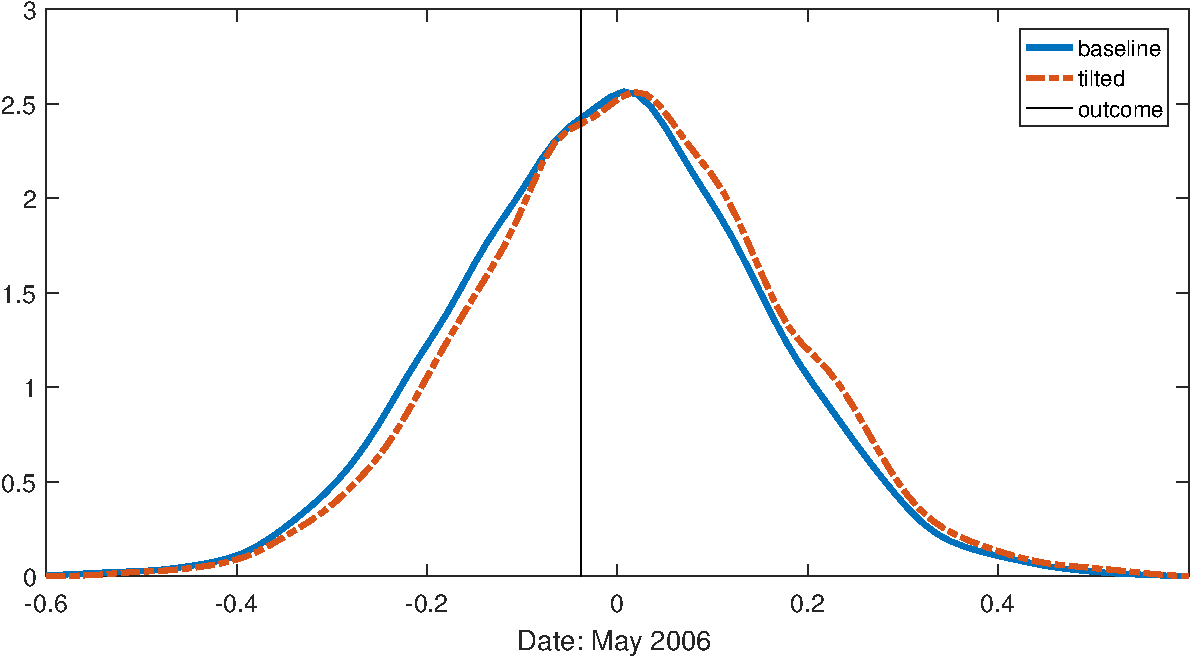
\includegraphics[width=0.49\linewidth]{../../Tex/plots/IBM_density_m1}
		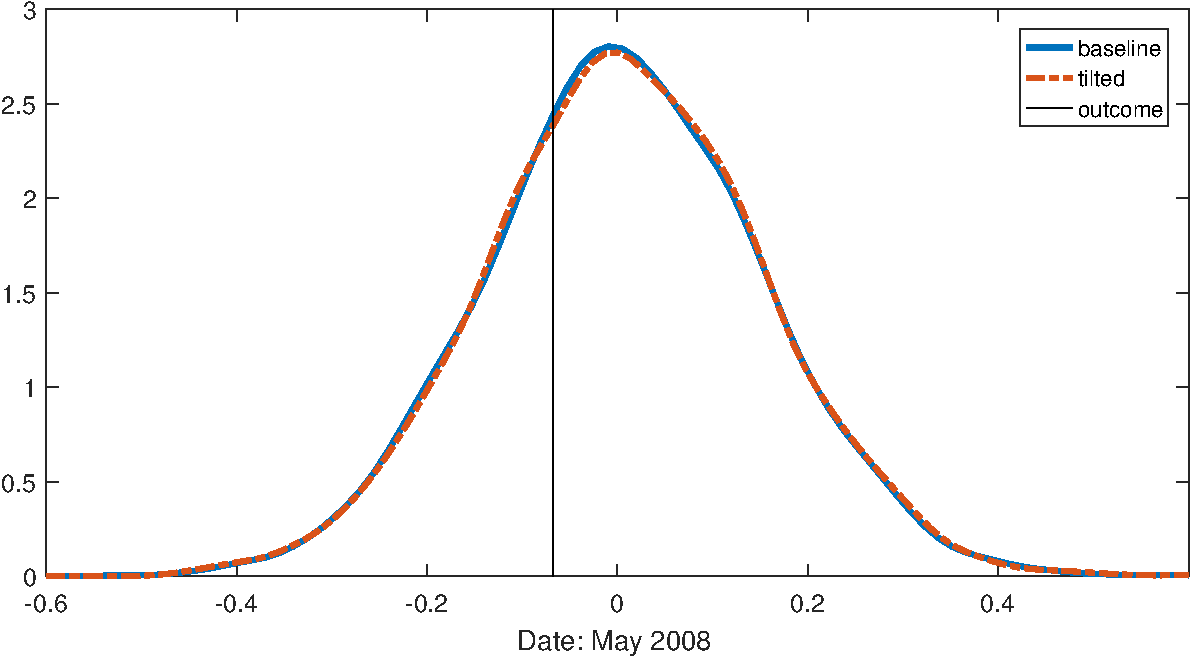
\includegraphics[width=0.49\linewidth]{../../Tex/plots/IBM_density_m2}\\
		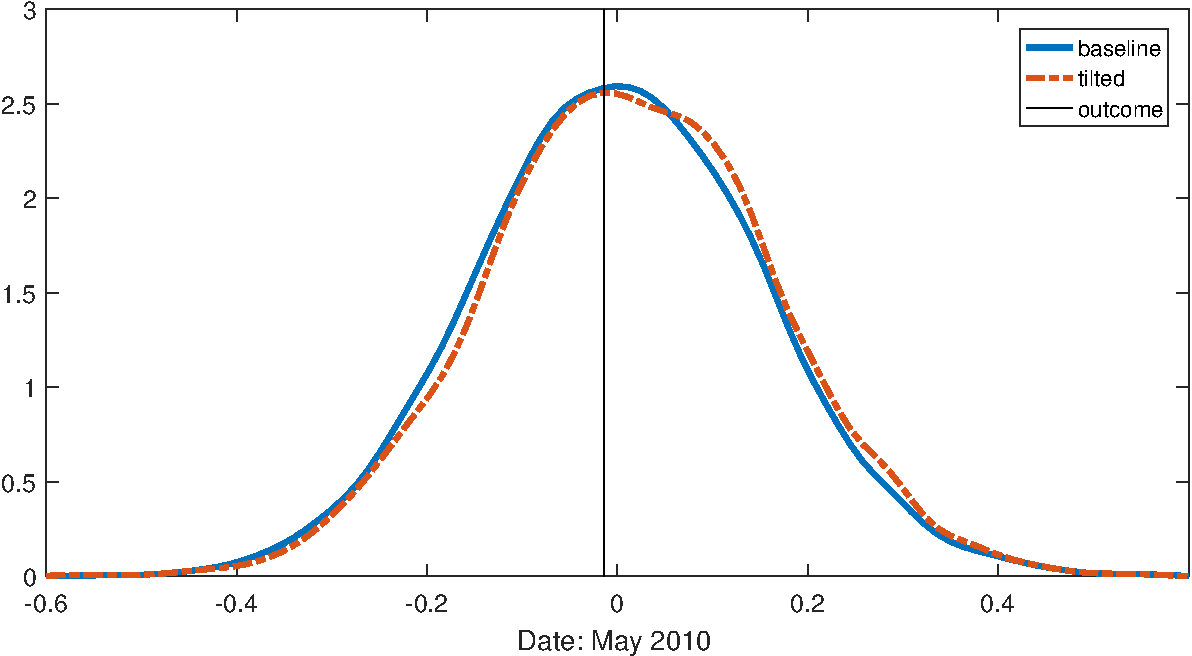
\includegraphics[width=0.49\linewidth]{../../Tex/plots/IBM_density_m3}
		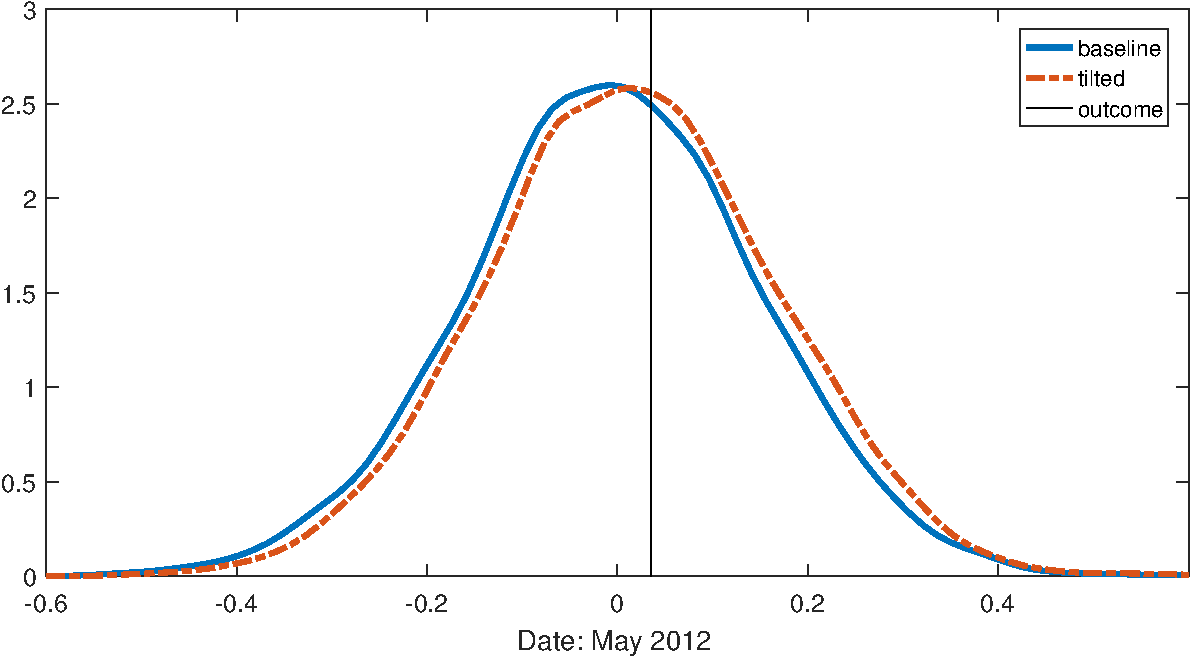
\includegraphics[width=0.49\linewidth]{../../Tex/plots/IBM_density_m4}
		\label{fig:ibmdensplotm}
	\end{figure}
\end{frame}
%%%%%%%%%%%%%%%%%%%%%%%%%%%
%%%%%%%%%%%%%%%%%%%%%%%%%%%

\begin{frame}{Kernel Predictive Densities - IBM - Mean/Variance Tilting}
	\begin{figure}
		\centering
		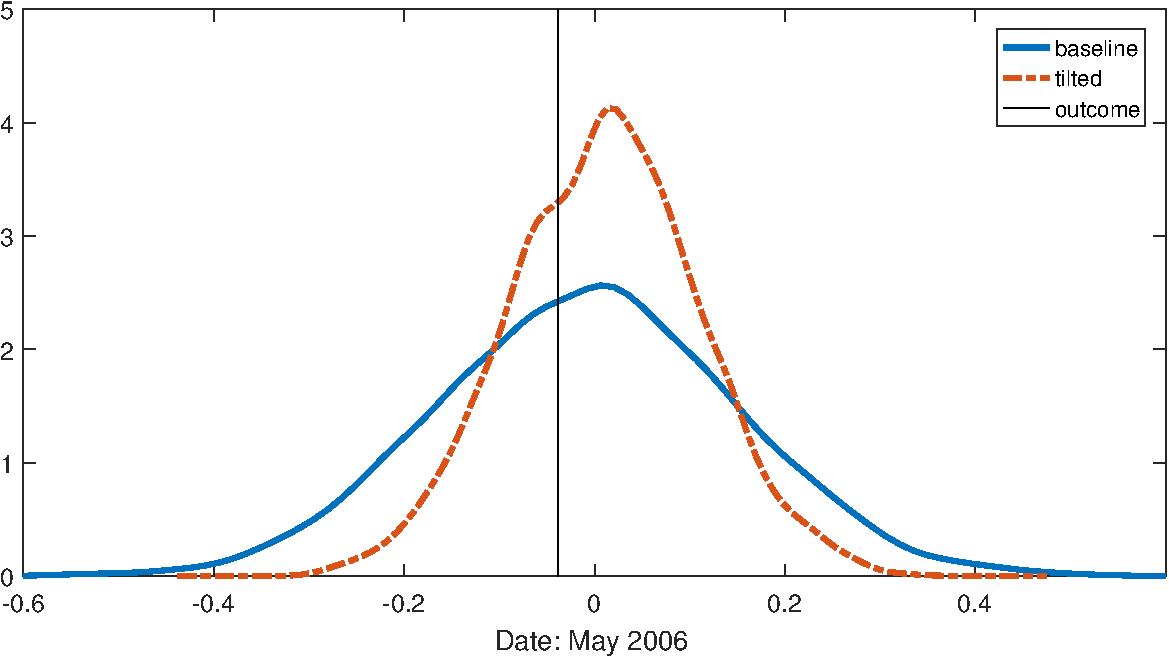
\includegraphics[width=0.49\linewidth]{../../Tex/plots/IBM_density_mv1}
		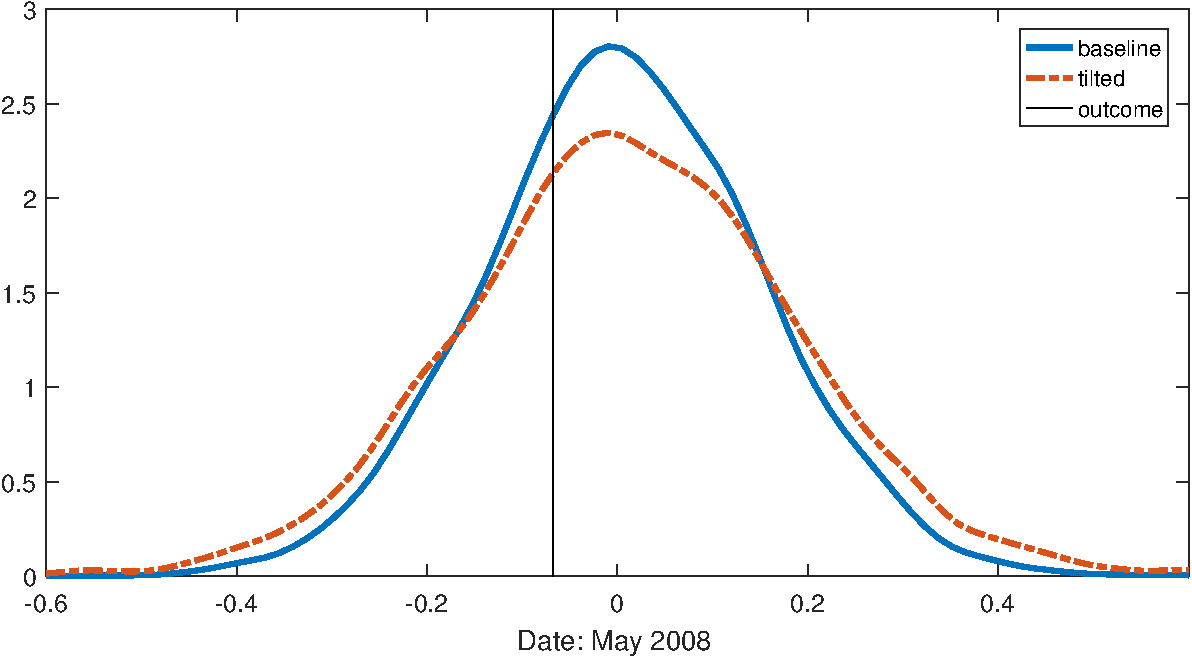
\includegraphics[width=0.49\linewidth]{../../Tex/plots/IBM_density_mv2}\\
		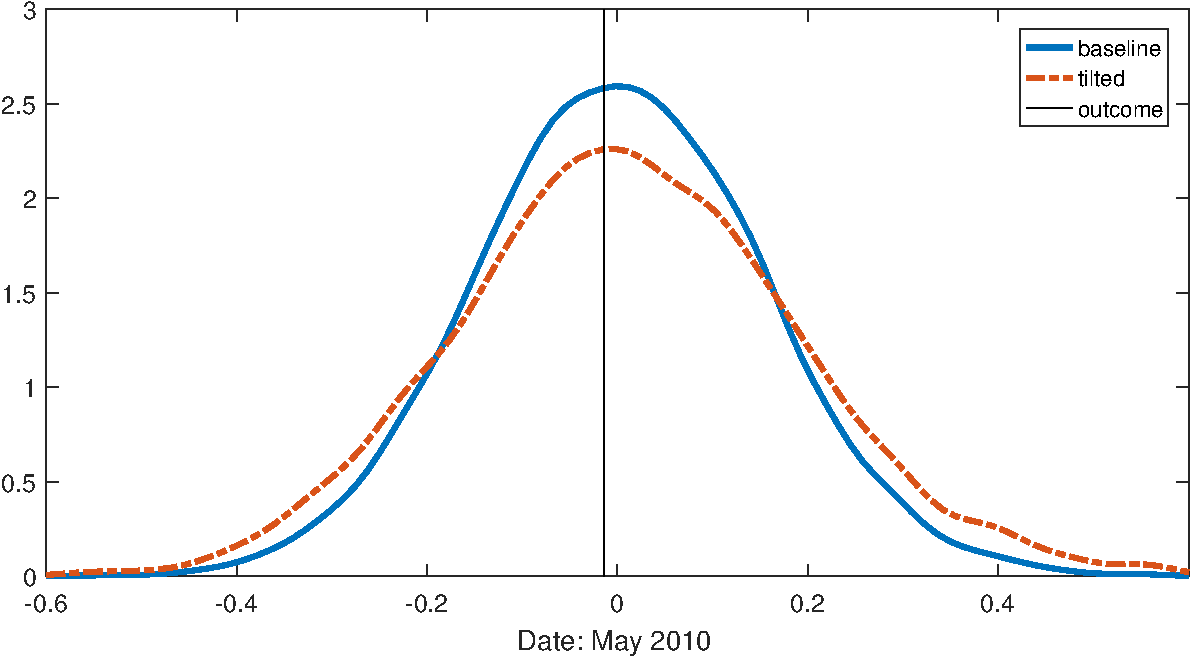
\includegraphics[width=0.49\linewidth]{../../Tex/plots/IBM_density_mv3}
		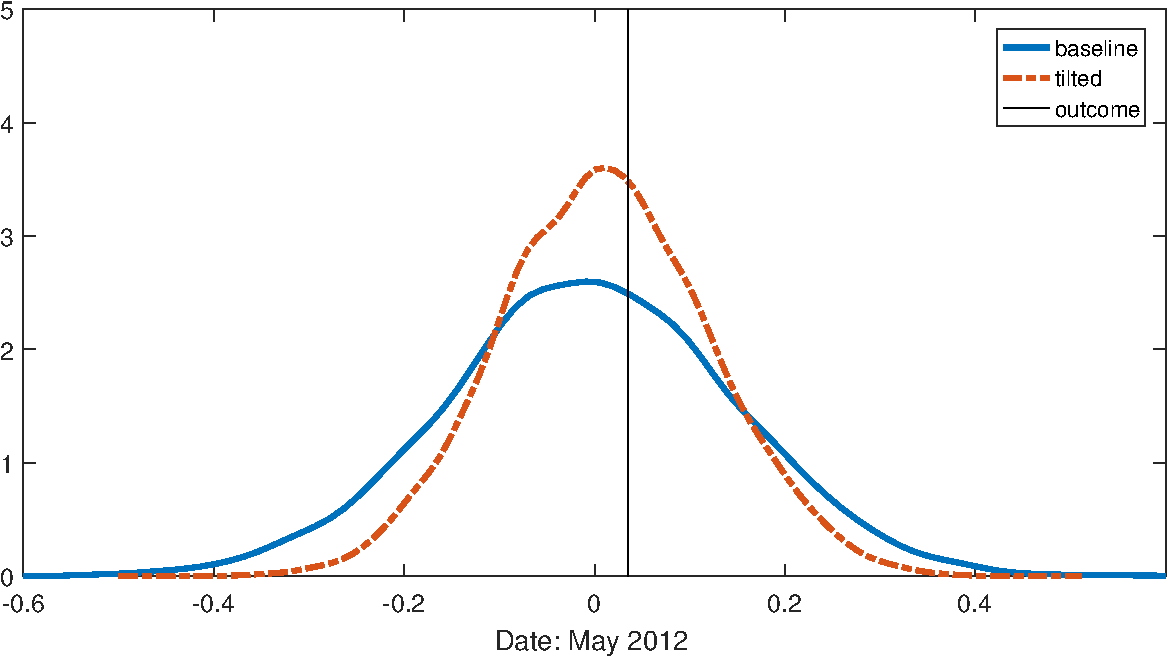
\includegraphics[width=0.49\linewidth]{../../Tex/plots/IBM_density_mv4}
		\label{fig:ibmdensplotmv}
	\end{figure}
\end{frame}
%%%%%%%%%%%%%%%%%%%%%%%%%%%
%%%%%%%%%%%%%%%%%%%%%%%%%%%

\section{Conclusions}

\begin{frame}{Conclusions and Outlook}
	\begin{itemize}
		\item We demonstrate that financial analyst forecasts can have predictive power for equity assets of the Dow Jones Industrial index
		\item Extent of predictability varies across assets but using Bayesian VARs with time-varying coefficients, stochastic volatility and model averaging and selection among priors improves return predictions across all assets
		\item Tilting the mean of the predictive distribution towards the target price implied expected returns does not improve forecast performance, but tilting mean and variance of the predictive return distribution improves forecasts
		%\item Advantage of entropic tilting: incorporate any kind of (forward-looking) information into a predictive regression framework in a parsimonious way without increasing estimation noise
	\end{itemize}
\pause
\textbf{Possible extensions:}
\begin{itemize}
	\item Relax assumption of strict moment conditions
	\item Panel VAR systems for various assets to model joint predictive return distributions for finding optimal portfolios
	\item Apply the tilting framework to predictive portfolio weight regressions \citep{frey2016a}
\end{itemize}
\end{frame}
%%%%%%%%%%%%%%%%%%%%%%%%%%%
%%%%%%%%%%%%%%%%%%%%%%%%%%%

%\begin{frame}{Outlook}
%\textbf{Possible extensions:}
%\vspace{0.5cm}
%\begin{itemize}
%	\item Relax assumption of strict moment conditions
%	\item Panel VAR systems for various assets to model joint predictive return distributions for finding optimal portfolios
%	\item Apply the tilting framework to predictive portfolio weight regressions \citep{frey2016a}
%\end{itemize}
%\end{frame}
%%%%%%%%%%%%%%%%%%%%%%%%%%%%
%%%%%%%%%%%%%%%%%%%%%%%%%%%%

\appendix
\newcounter{finalframe}
\setcounter{finalframe}{\value{framenumber}}


\begin{frame}[plain]{References}
\fontsize{5}{5}\selectfont{
	\setlength{\bibsep}{0\baselineskip}
	\bibliographystyle{ecta}
	\bibliography{./tilting}}
\end{frame}
%%%%%%%%%%%%%%%%%%%%%%%%%%%
%%%%%%%%%%%%%%%%%%%%%%%%%%%

\begin{frame}[plain]{Motivation - IBM Stock Price II}
\begin{itemize}
	\item Mean target price $\pm$ 1.96 $\times$ S.D. of target prices 
\end{itemize}

\begin{figure}
	\centering
	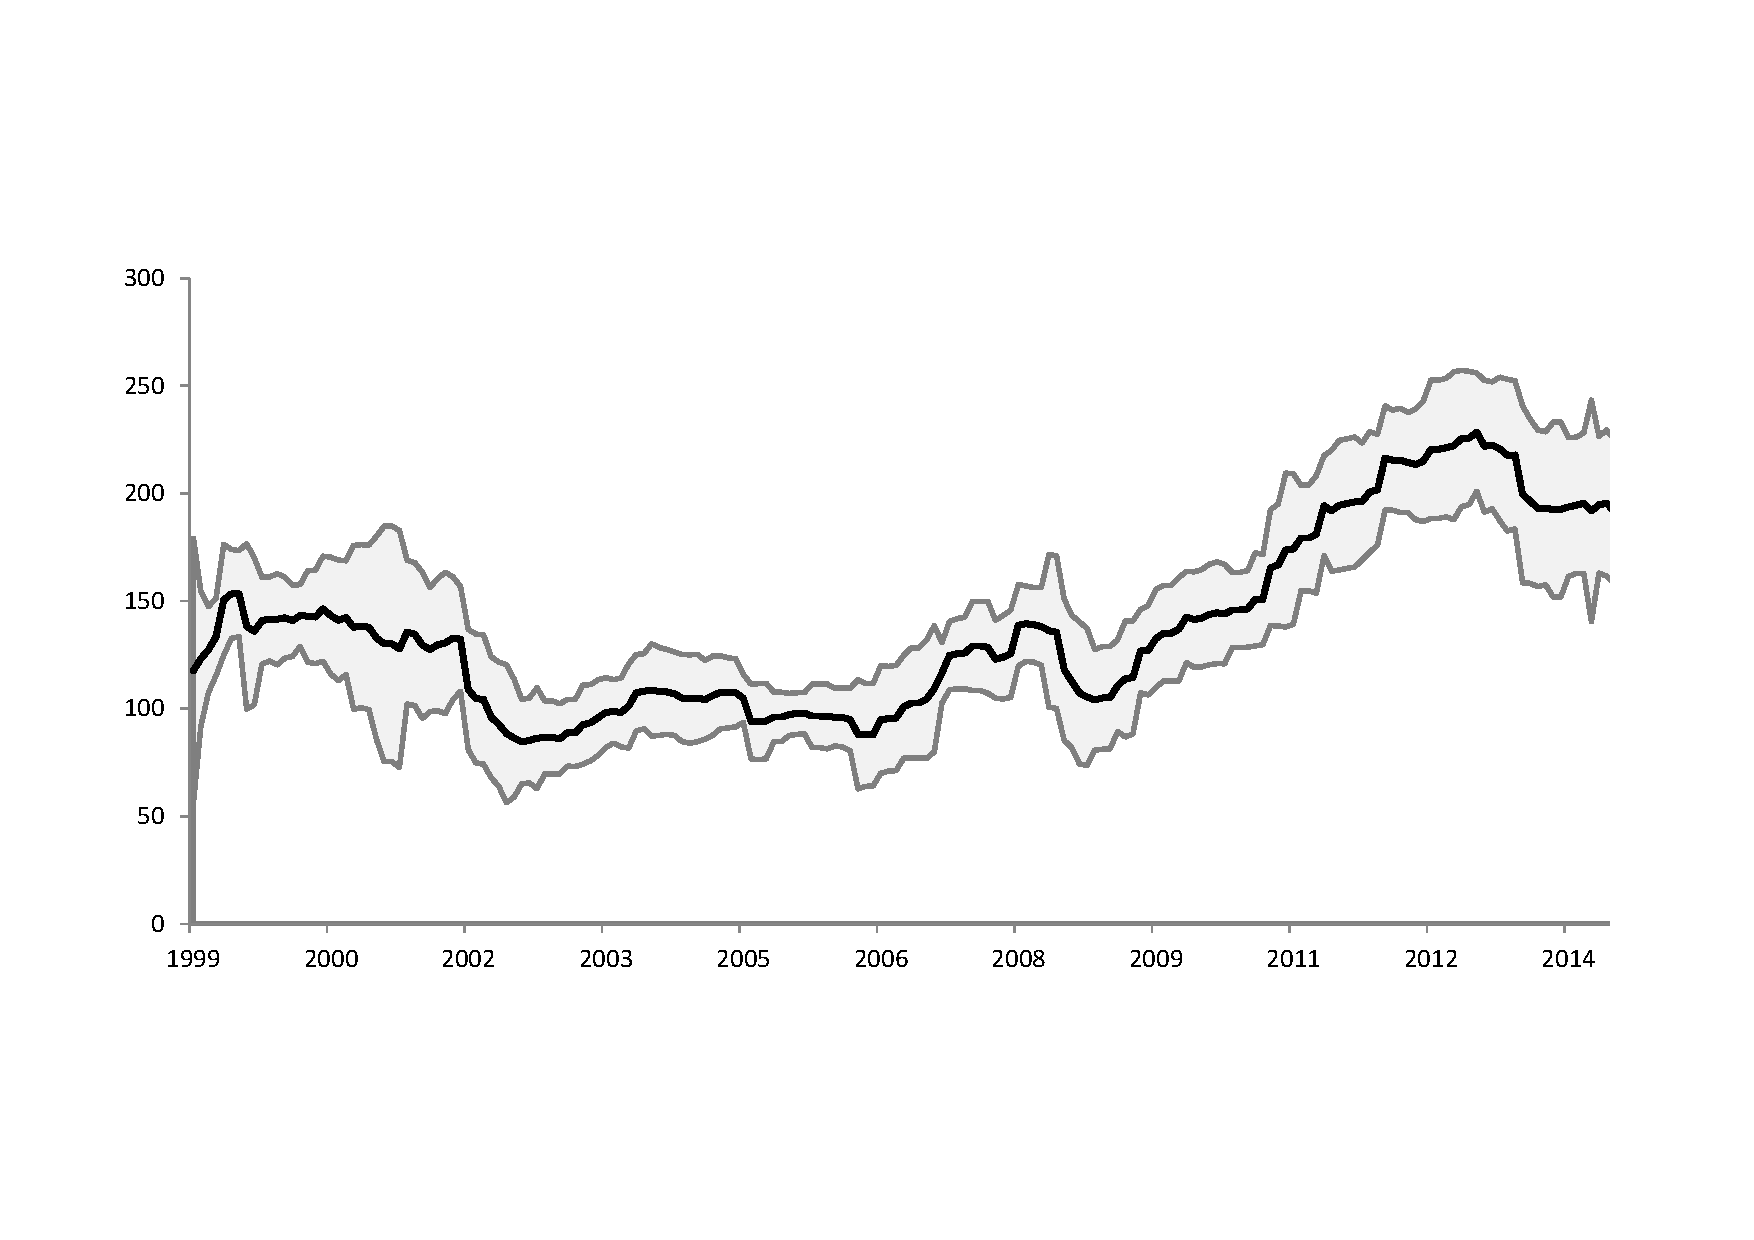
\includegraphics[width=1\linewidth]{../../Tex/plots/ibm_SD}
	\label{fig:ibmpriceplot}
\end{figure}

\end{frame}
%%%%%%%%%%%%%%%%%%%%%%%%%%%
%%%%%%%%%%%%%%%%%%%%%%%%%%%

\begin{frame}[plain]{Predictor variables}
\begin{itemize}\setlength\itemsep{1em}
	\item Company specific: Log DY, Log EPR, Log DPR, BMR, 
	\item Macroeconomic: 3M Tbill rate, Longterm yield, Market return, CPI inflation
	\item Analyst information: Log TPR, Log TPRV, Log REC, Log REC return
\end{itemize}
\end{frame}
%%%%%%%%%%%%%%%%%%%%%%%%%%%
%%%%%%%%%%%%%%%%%%%%%%%%%%%

\setcounter{framenumber}{\value{finalframe}}

\end{document}
